\chapter{\texorpdfstring{The \nova~Experiment}{The NOvA Experiment}}
\label{ch:nova}

The \nova~experiment, or the NuMI Off-Axis $\nue$ Appearance experiment, is a long baseline, two detector, neutrino oscillation experiment designed to measure $\numu$ to $\nue$ appearance from the Fermilab NuMI beam. The two functionally identical \nova~detectors are situated $14.6\unit{mrad}$ off-axis of the beam center, with its Near Detector (ND) located approximately $1\unit{km}$ downstream of the beam target source and its Far Detector (FD) located $810\unit{km}$ from the source in Ash River, MN. The main purpose of the ND is to constrain the neutrino beam energy and composition by measuring the beam very close to its source, i.e., before the neutrinos have had a chance to oscillate. The FD then measures the oscillated neutrinos. This chapter describes the NuMI beam and \nova~detectors in more detail.

\section{The NuMI Beam}
\label{sec:NuMI}

The NuMI beam is a $\numu$ beam generated at Fermi National Accelerator Laboratory, or Fermilab, in Batavia, IL, and the source of neutrinos for the \nova~experiment. The neutrino beam is created by accelerating protons to $120\unit{GeV}$, colliding them with a graphite target, and allowing the products to decay to neutrinos.

The NuMI beam originates with the $120\unit{GeV}$ protons, and these are accelerated in the complex shown in figure \ref{fig:FNAL_AC}. First, negatively charged hydrogen atoms are accelerated to $400\unit{MeV}$ in the Linac. These atoms next enter the Booster synchrotron where the electrons are removed and the protons are accelerated to $8\unit{GeV}$. The output of from the booster is $13$ bunches, $12$ which are extracted into the Recycler Ring, each with approximately $4\times10^{12}$ protons. In a procedure called slip stacking, additional bunches are used to double the intensity of each bunch. The first bunches in the Recycler are decelerated slightly while $6$ new bunches enter the ring. As the two sets of bunches have slightly different energies, they slip relative to each other. When two bunches overlap they are captured with a special RF pulse, creating $6$ larger bunches that are extracted into the Main Injector (MI) and accelerated to $120\unit{GeV}$. Finally, these protons are directed to a target for neutrino production. At this point, the 6 bunches, or the spill, total about $5\times10^{13}$ protons. With a cycle time of $1.333\unit{s}$, the NuMI beam reaches $700\unit{kW}$, which is the most powerful beam in the world \cite{ref:TDRNOvA}.
\begin{figure}[htb]
  \centering
  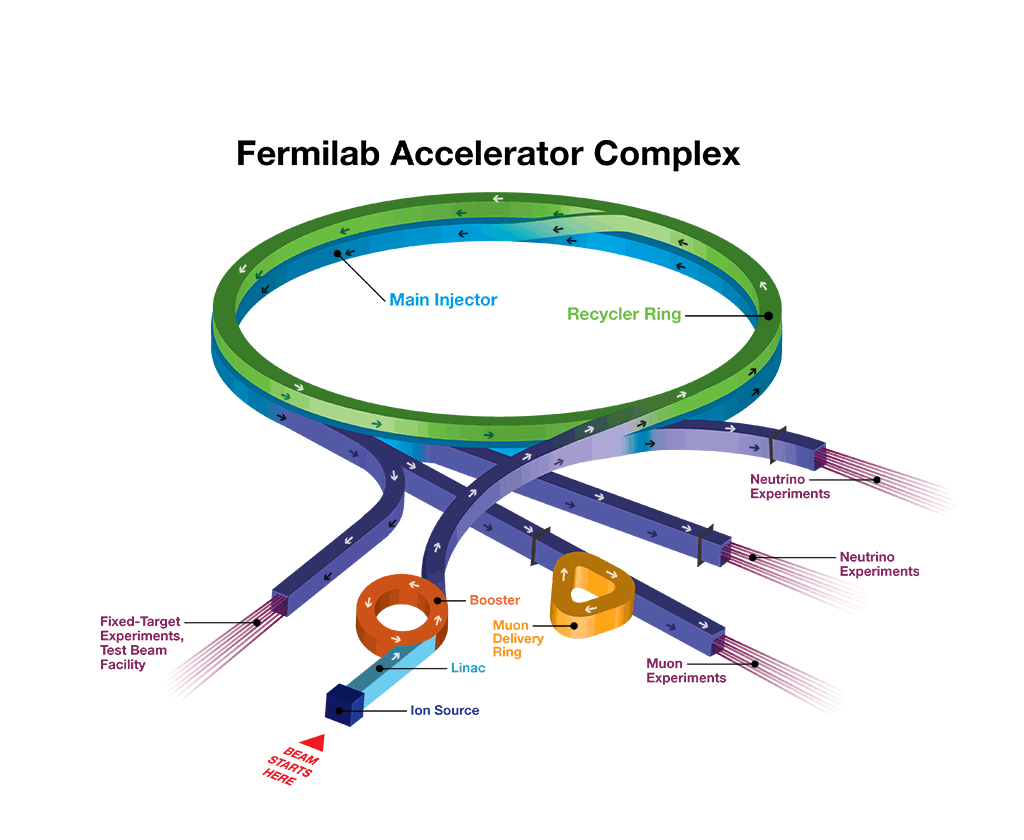
\includegraphics[width=0.75\textwidth]{figures/FNAL_AC.png}
  \caption[Fermilab Accelerator Complex]{Schematic of the Fermilab accelerator complex.}
  \label{fig:FNAL_AC}
\end{figure}

In truth, the above is the design goal of the NuMI beam upgrades. The NuMI beam was originally designed for the MINOS experiment \cite{ref:TDRNuMI}, and it was operating at ${\sim}200\unit{kW}$ with no slip stacking at the time of writing the \nova~Technical Design Report (TDR) in 2007 \cite{ref:TDRNOvA}. Since then, the Fermilab Accelerator Division has been steadily ramping up the beam power, as shown in figure \ref{fig:BeamPower}. At the time of writing of this dissertation, the NuMI beam was in the midst of its 2016 summer shutdown. Before the beam was powered down, it most recently was running stably at about $560\unit{kW}$ with $6{+}4$ slip stacking, or doubling the proton intensity in just $4$ of $6$ bunches \cite{ref:IntensitykW, ref:IntensitySlip}. However, the NuMI beam briefly reached its design goal of $700\unit{kW}$ with full $6{+}6$ slip stacking during a test on June 13, 2016 \cite{ref:Intensity700}.
\begin{figure}[htb]
  \centering
  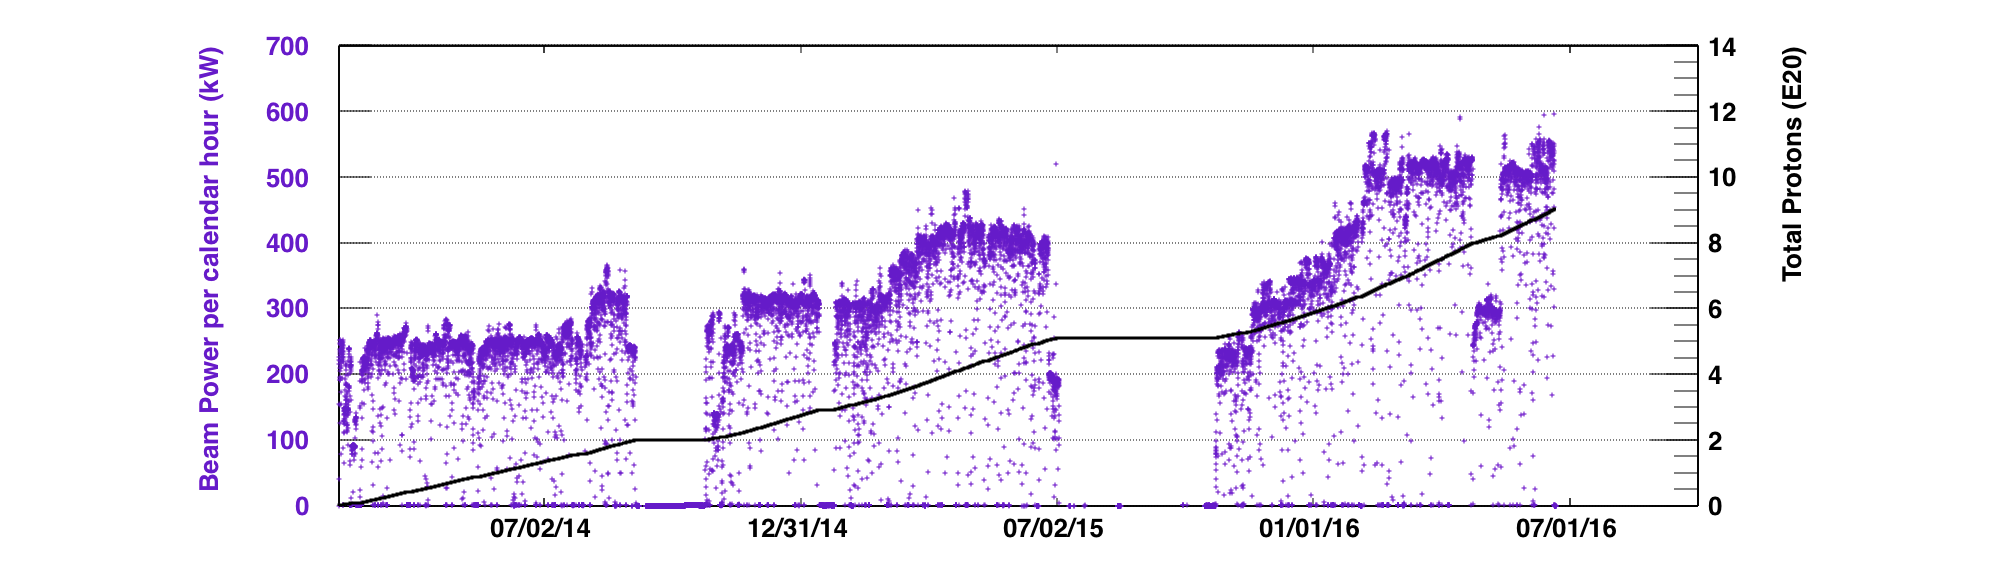
\includegraphics[width=1\textwidth]{figures/BeamPower.png}
  \caption[Beam Power vs Time]{Beam power vs time since \nova~began collecting data. The average beam power is shown as purple points, and the integrated POT is shown in the black curve.}
  \label{fig:BeamPower}
\end{figure}

To generation of the actual neutrino beam begins with the extraction of the $120\unit{GeV}$ protons from the MI into the complex shown as a schematic in figure \ref{fig:FNAL_NuMI}. The protons are directed $3.3^\circ$ downward into the earth so the NuMI beam points directly toward the MINOS FD in Soudan, MN. First the protons collide with atoms inside a long, thin target. The target consists of 47 graphite `fins' that are each $20.0\unit{mm}$ long, $6.4\unit{mm}$ wide, and spaced $0.3\unit{mm}$ apart for a total length of $95.4\unit{cm}$. The beam size at the target is $1\unit{mm} \times 1\unit{mm}$, and the length of the target corresponds to ${\sim}2$ interaction lengths for the protons \cite{ref:TDRNuMI}. \nova~performs its data accounting by summing the protons on target, or POT. The interactions in the target produce a large number of secondary hadrons consisting mainly of charged pions with a smaller contribution of kaons. These particles next pass through two magnetic, parabolic horns. A current of $200\unit{kA}$ is passed through the horns creating a $1/r$ magnetic field that focuses a one sign of the charged particles and defocuses the opposite sign. The current in the horns can be reversed, which allows the NuMI beam to run in either neutrino or antineutrino mode. When positively charged particles are focused, they decay into neutrinos, and similar for negatively charged particles and antineutrinos. Next, the focused charged particles travels through a $675\unit{m}$ long, $1\unit{m}$ radius decay pipe where the hadrons decay into neutrinos and tertiary charged leptons \cite{ref:TDRNOvA}. Finally, everything passes through a hadron monitor and absorber followed by three muon monitors spaced between sections of rock, leaving only the neutrinos to reach the ND hall.
\begin{figure}[htb]
  \centering
  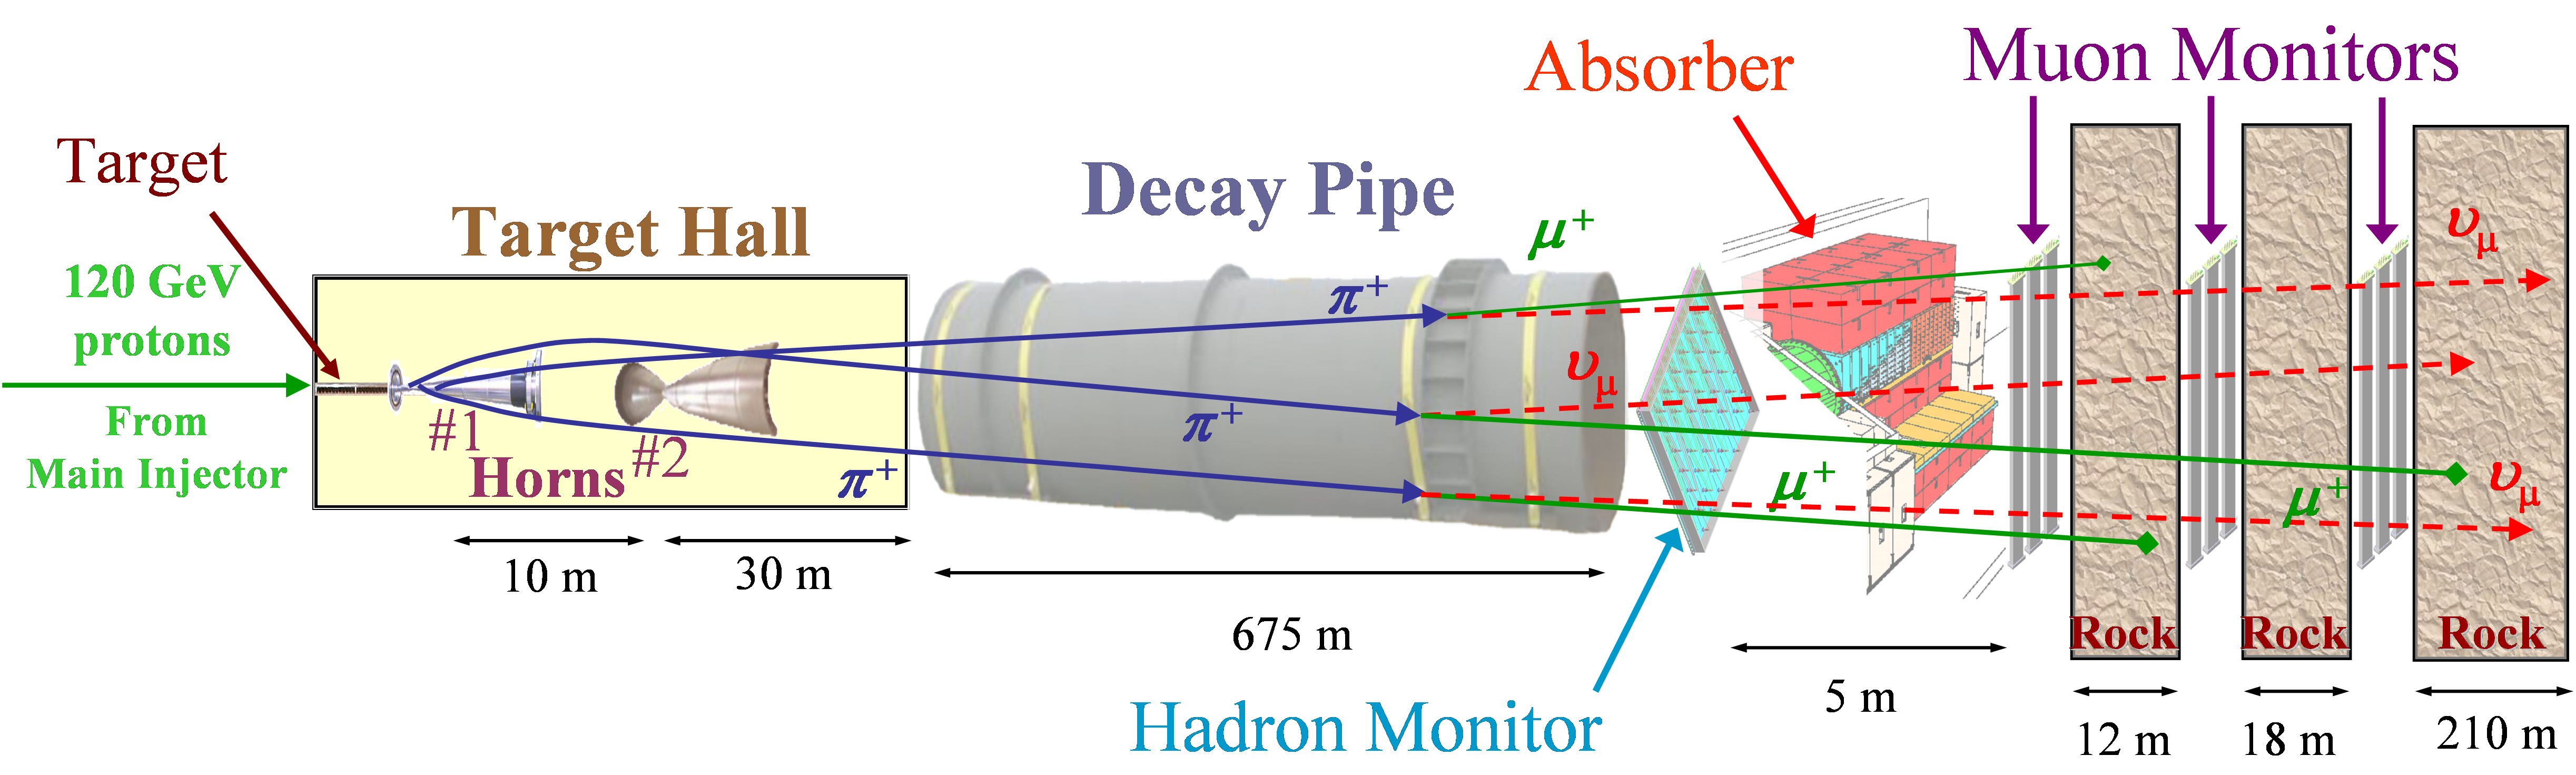
\includegraphics[width=1\textwidth]{figures/FNAL_NuMI.png}
  \caption[NuMI Beam Schematic]{Schematic of the NuMI beam.}
  \label{fig:FNAL_NuMI}
\end{figure}

As a final note for this section, all of the data analyzed in this dissertation was taken during neutrino mode running, so the anti-neutrino mode is not considered further.

\section{Off-Axis Detectors}

The \nova~experiment was designed to have its detectors located $14.6\unit{mrad}$ off-axis from the NuMI beam, and this greatly affects the observed neutrino energy spectrum. The main decay mode for charged pions ($99.98770\%$) and kaons ($63.56\%$) is the two body decay into a muon and muon-neutrino \cite{ref:PDG}. In the center of mass frame of the decaying meson, this is a deterministic, isotropic decay. However, the lab frame is highly boosted resulting in the following neutrino flux and energy spectrum for a detector with cross section area $A$ located a distance $L$ from the decay point.
\beqa
\phi_\nu & = & \left( \frac{2\gamma_m}{ 1 + \gamma^2_m \theta^2 } \right)^2 \frac{A}{4\pi L^2} \label{eq:OffAxisFlux} \\
E_\nu & = & \left(1 - \frac{m^2_\mu}{m^2_m} \right) \frac{E_m}{1 + \gamma^2_m \theta^2} \label{eq:OffAxisE}
\eeqa

\n Above, $\theta$ is the angle between the neutrino and meson, and the subscript $m$ refers to the decaying meson, i.e., $E_m$ is the meson energy, $m_m$ is the meson mass, and $\gamma_m$ is $E_m / m_m$. The effects of an off-axis location is shown in figure \ref{fig:OffAxis}. There are two competing effects that occur. While the flux of neutrinos is drastically reduced, the neutrino energy is highly constrained, with a net result of a very narrow band beam of neutrinos.
\begin{figure}[htb]
  \centering
  \begin{tabular}{c c}
    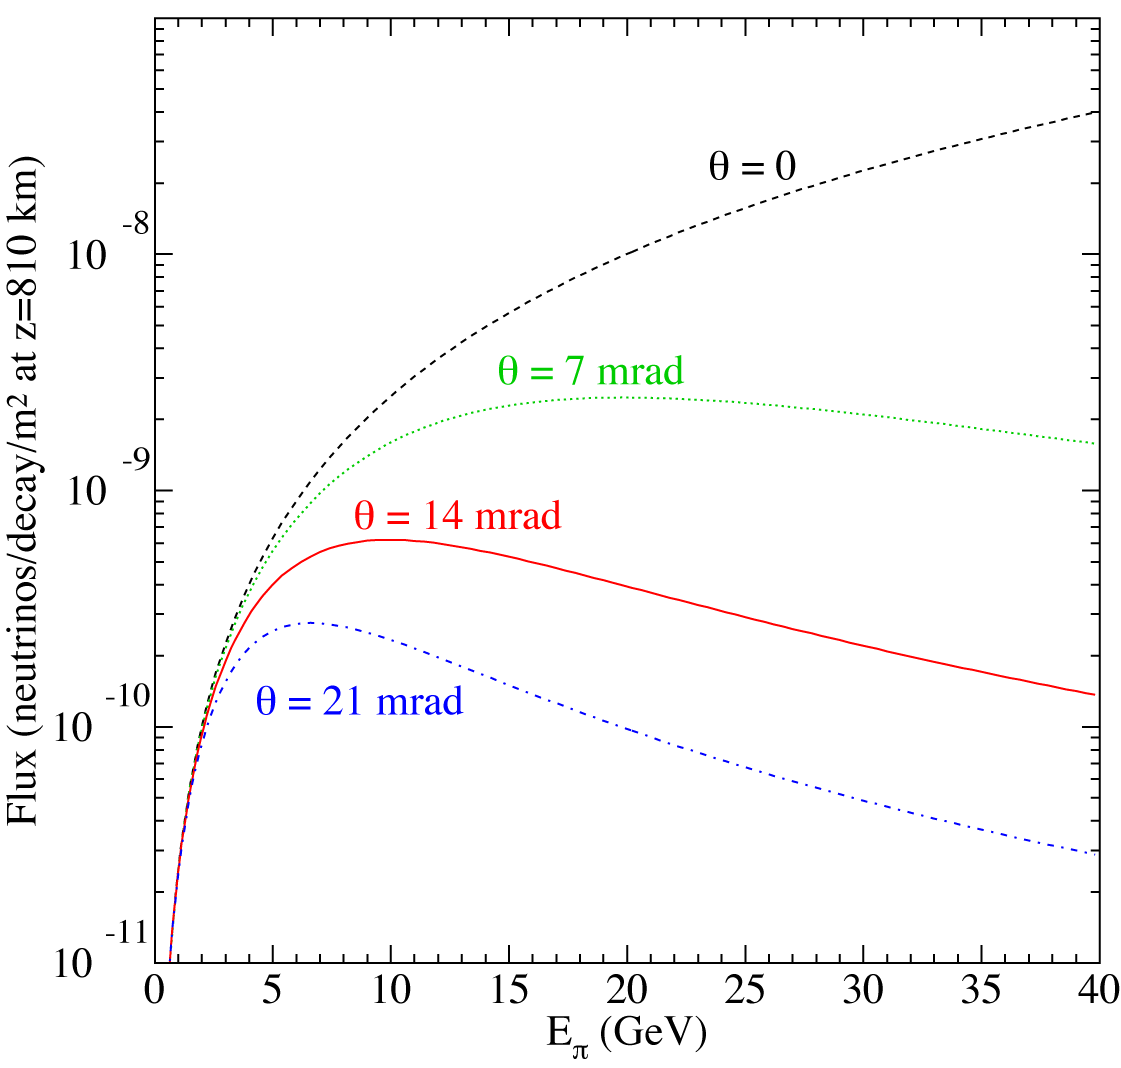
\includegraphics[width=.47\textwidth]{figures/OffAxisFlux.png} &
    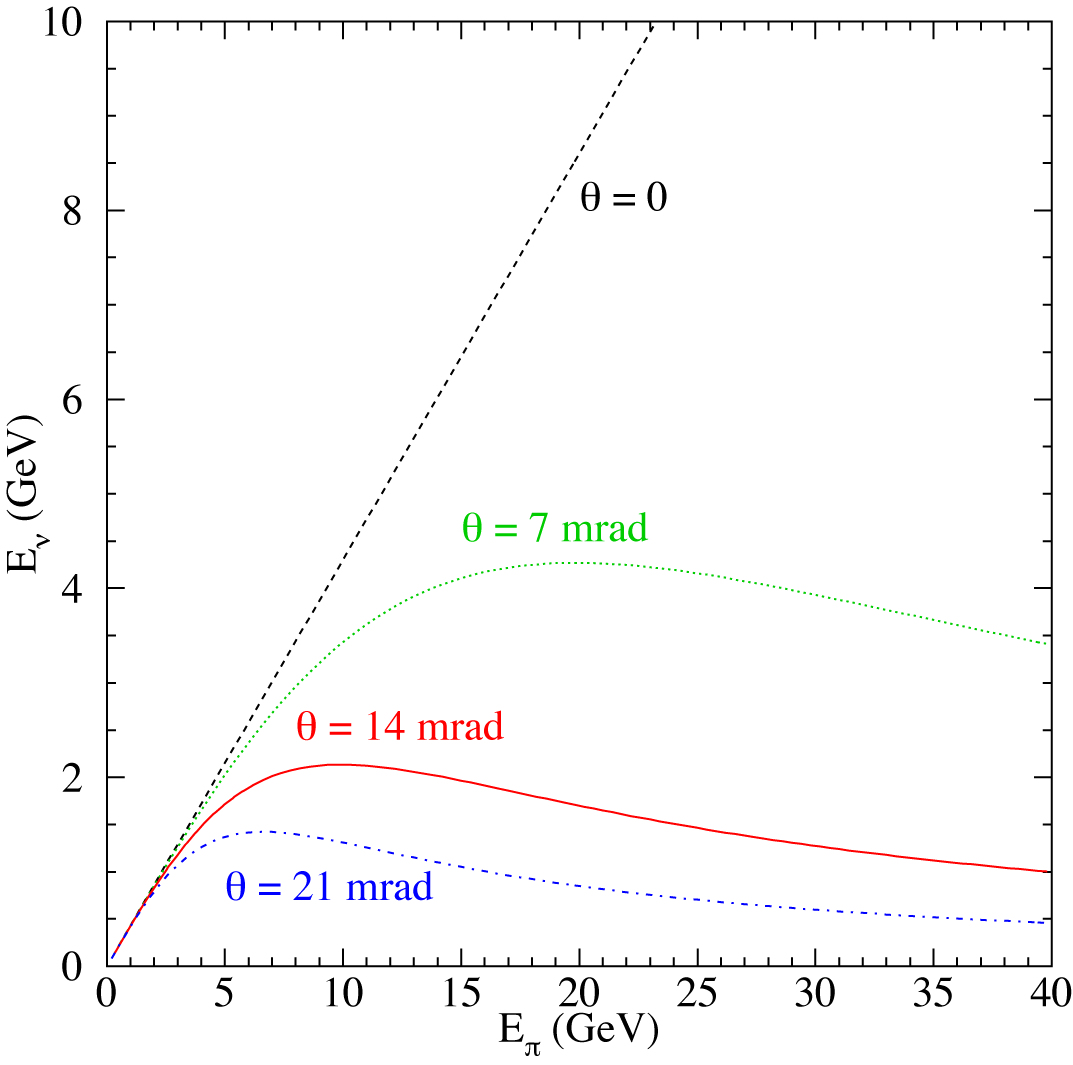
\includegraphics[width=.47\textwidth]{figures/OffAxisE.png} \\
  \end{tabular}
  \caption[Off-Axis Flux and Energy]{The neutrino flux (left) and energy (right) as a function of the decaying pion energy for several different off-axis angles. The on axis values are shown in black, and the red curves show the values for \nova. Plots from \cite{ref:TDRNOvA}}
  \label{fig:OffAxis}
\end{figure}

The narrow energy band result is shown in figure \ref{fig:BeamEComp}, which compares the energy spectrum for several off-axis angles and shows composition of the neutrino beam observed by \nova, both for the FD and without considering oscillations. The small contamination of $\anumu$, $\nue$, and $\anue$ components come from several effects. The focusing horns discussed in the previous section are unable to defocus the most energetic wrong sign mesons, which mostly contributes to the $\anumu$ component through the decay $\pi^- \rightarrow \anumu + \mu^-$. In the decay pipe, some of the muons from pion decay also decay, contributing to both the $\anumu$ and $\nue$ components. While most $K^+$ decay to $\numu$, a small fraction (5.07\% \cite{ref:PDG}) decay via $K^+ \rightarrow \pi^0 + e^+ + \nue$. There is a very small $\anue$ component that is largely due to $K_L$ decay.
\begin{figure}[htb]
  \centering
  \begin{tabular}{c c}
    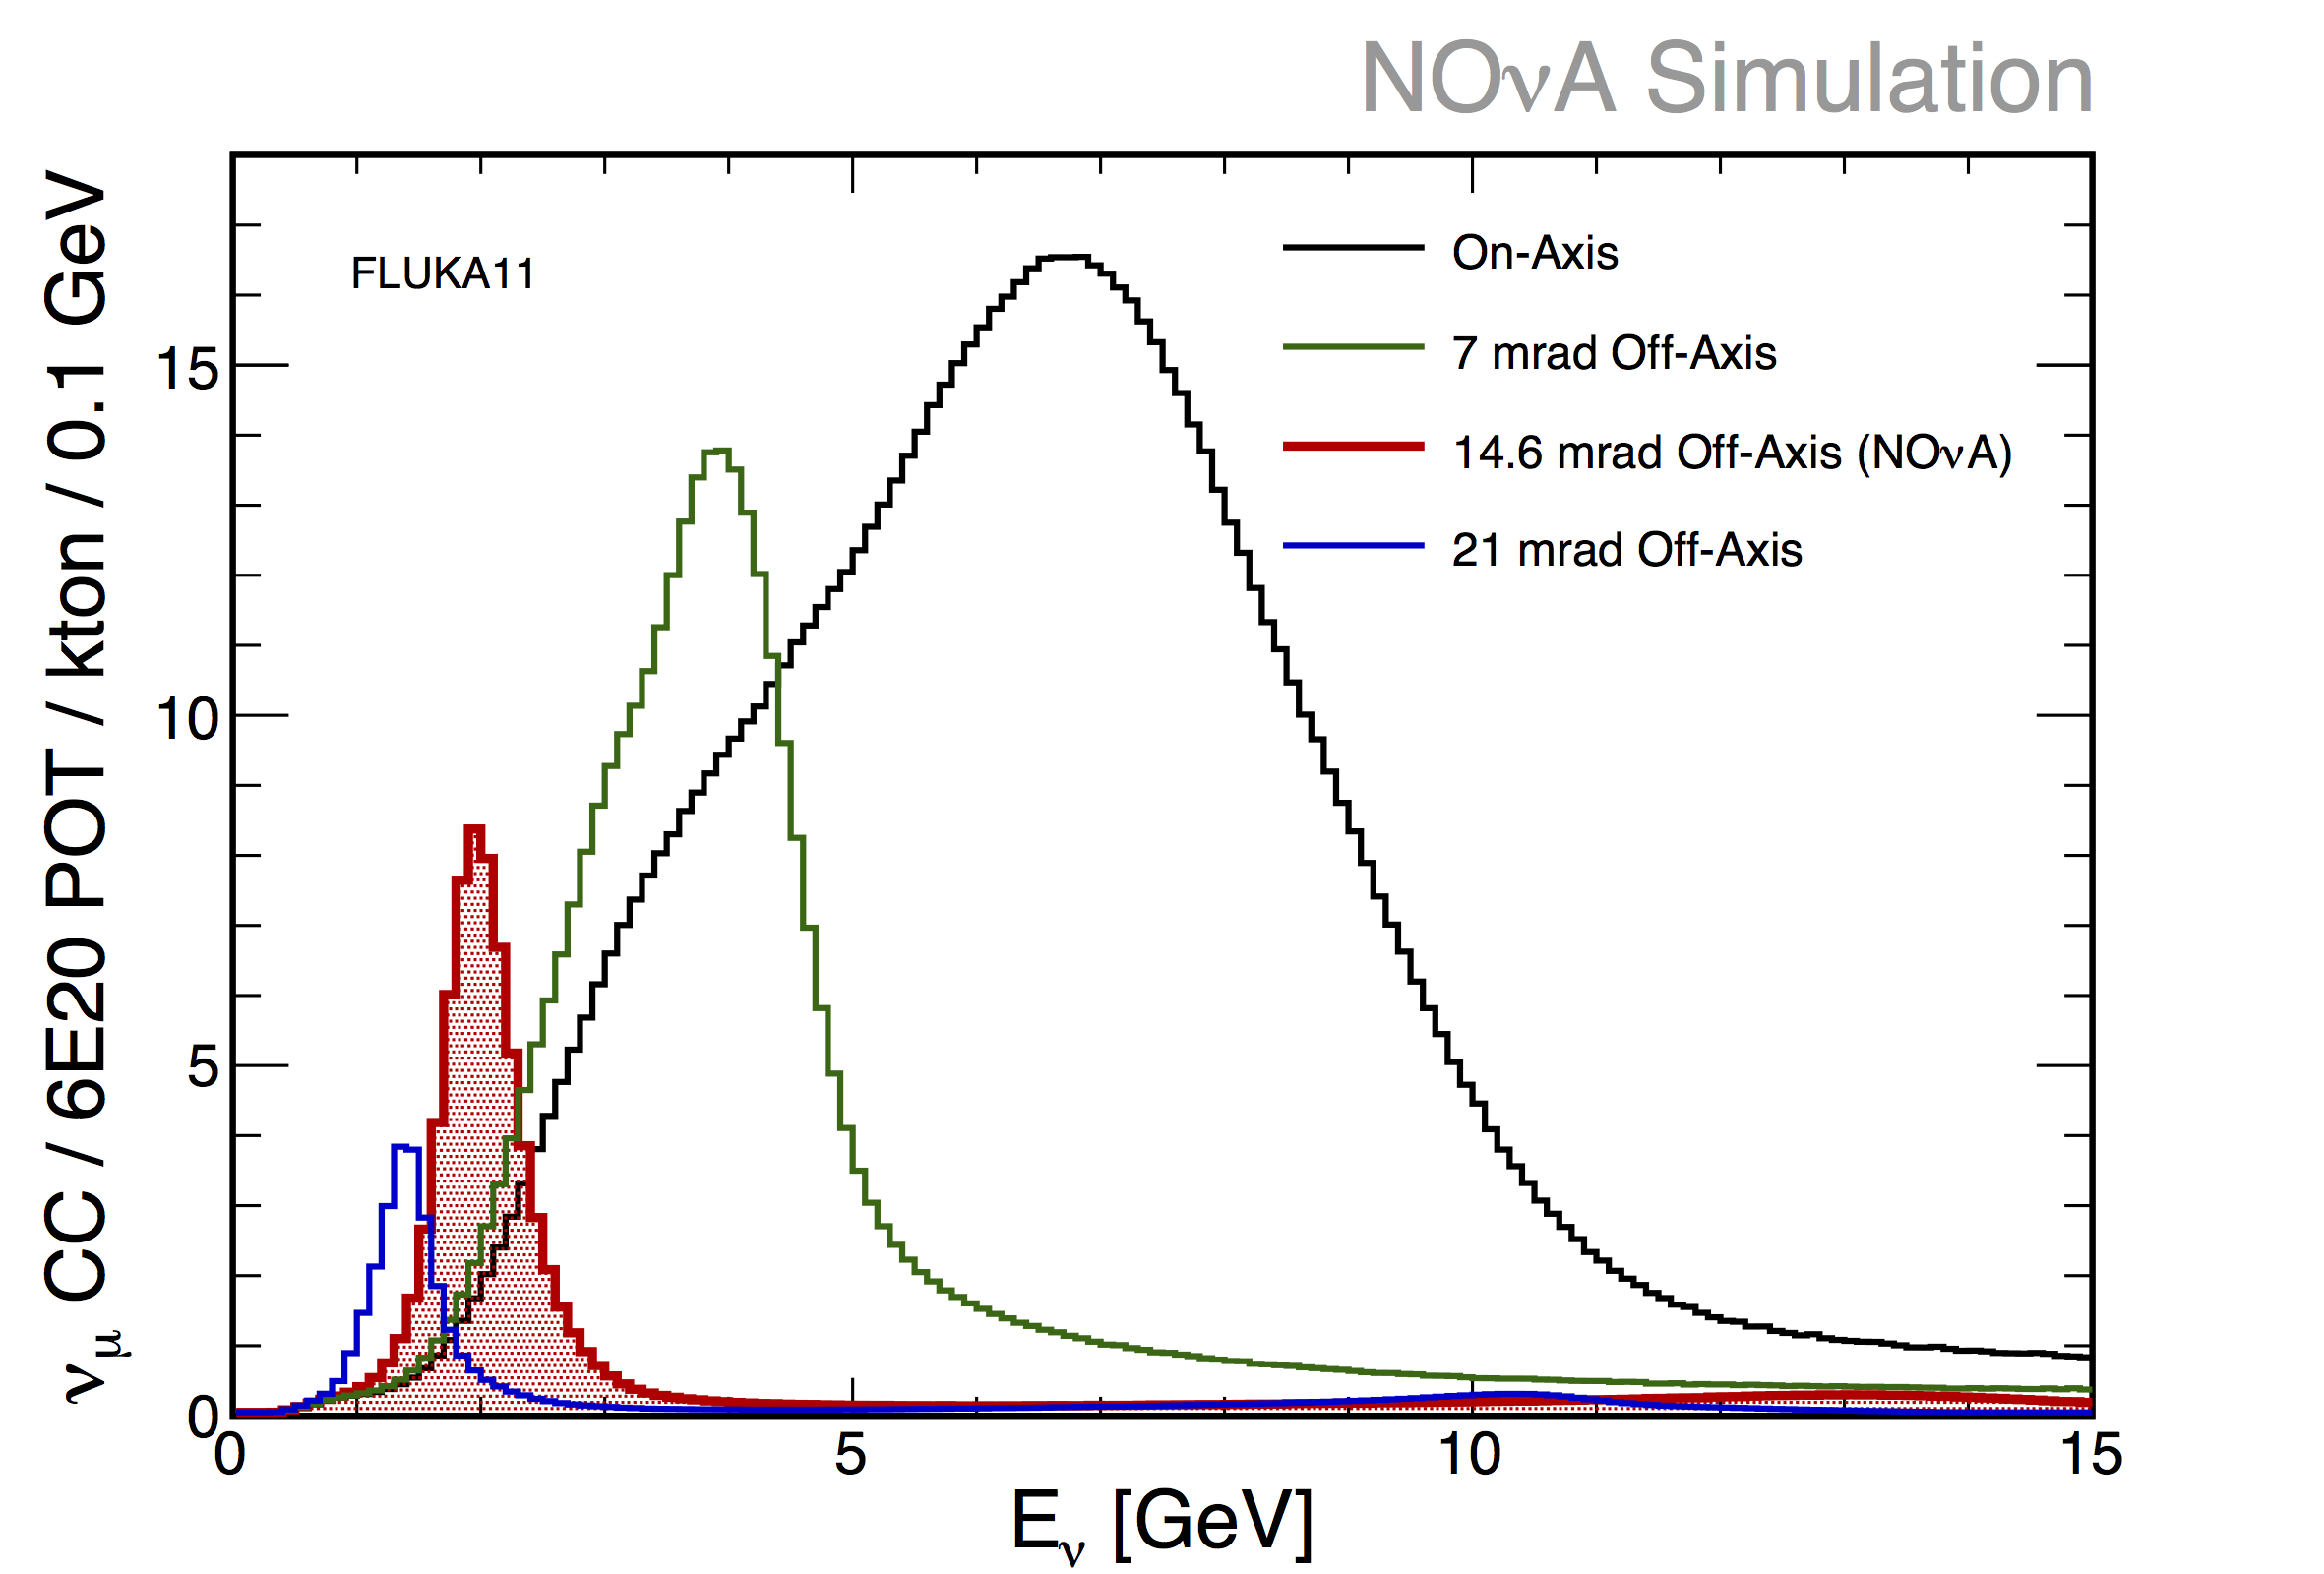
\includegraphics[width=.47\textwidth]{figures/BeamE.png} &
    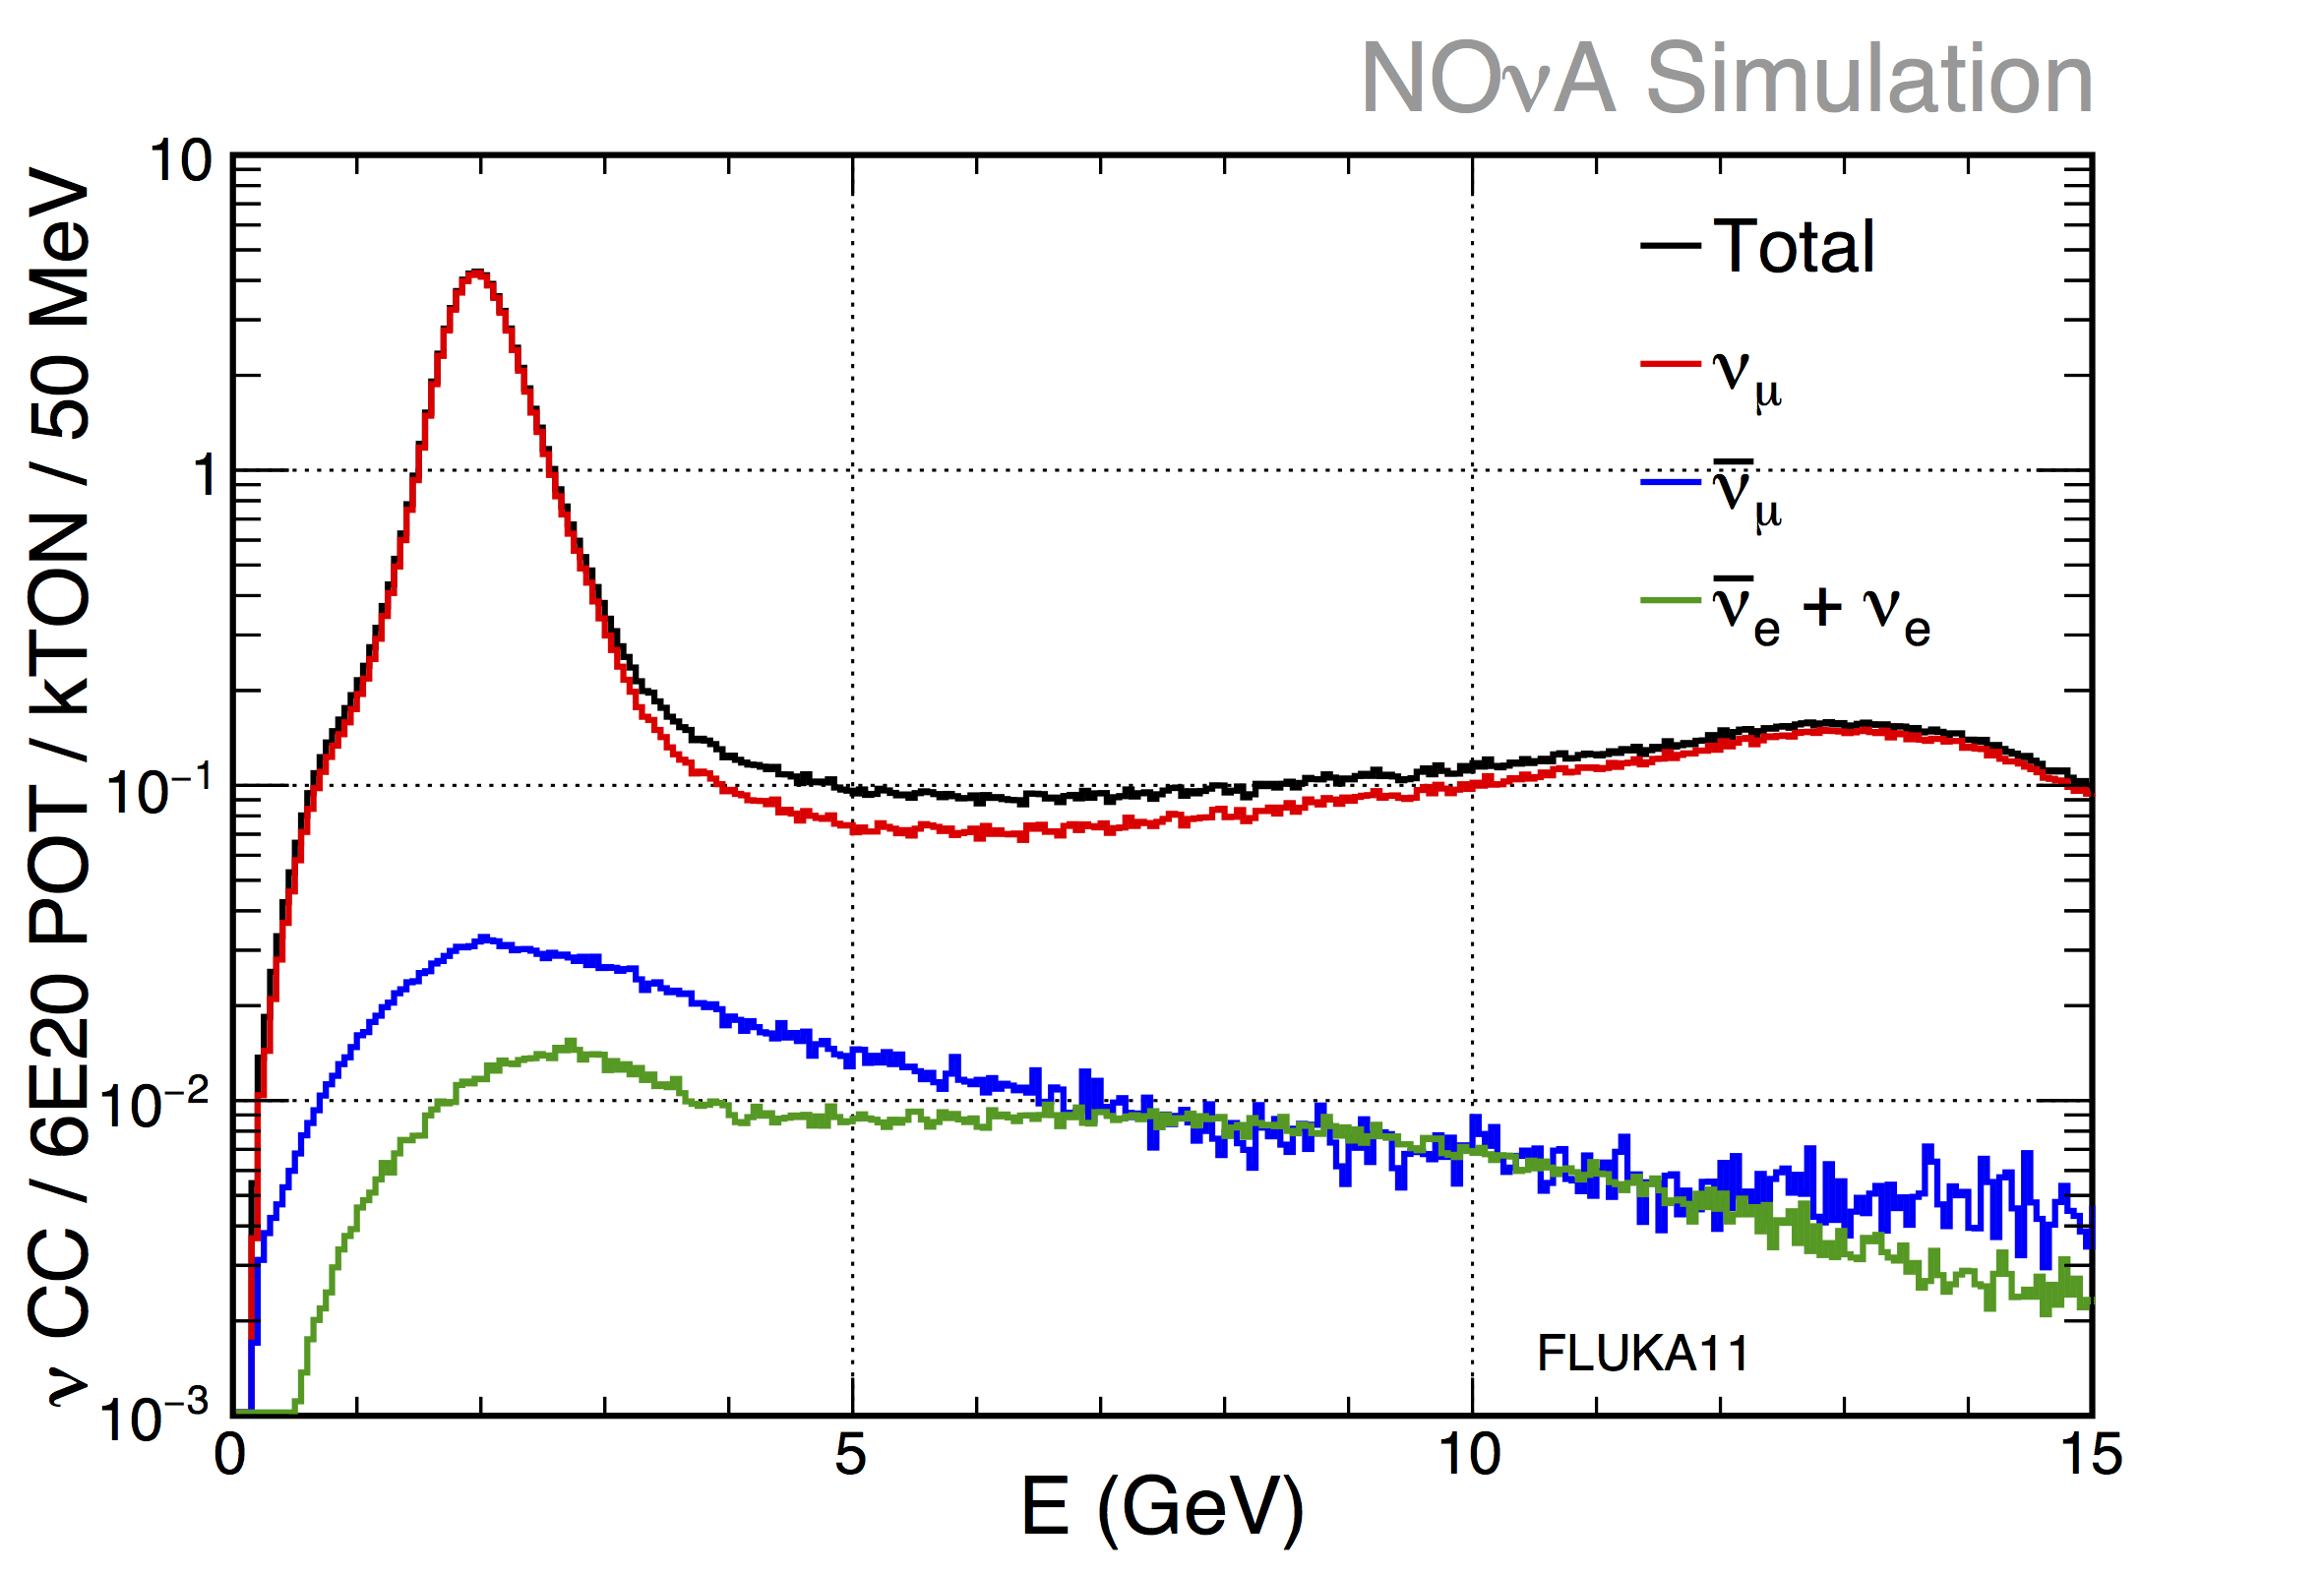
\includegraphics[width=.47\textwidth]{figures/BeamComp.png} \\
  \end{tabular}
  \caption[Beam Energy and Composition]{The neutrino flux (left) and energy (right) as a function of the decaying pion energy for several different off-axis angles. The on axis values are shown in black, and the red curves show the values for \nova.}
  \label{fig:BeamEComp}
\end{figure}

\nova~was designed to be off-axis in an attempt to optimize the amount of observed $\nue$ appearance, as the experiment name would suggest. At the \nova~FD, with $L = 810\unit{km}$, the neutrino energy range observed due to the particular off-axis angle falls right within the first oscillation maximum for $\nue$ appearance. Figure \ref{fig:PMuEFluxXSec} shows the oscillation probability for $\nue$ appearance and the event predictions for the dominant components, both as a function of the true neutrino energy. The narrow band beam and first oscillation peaks match quite well, allowing for the best possible measurement of $\nue$ appearance, one of \nova's two main analyses \cite{ref:NOvAFANuE}. Furthermore, the probability of $\numu$ disappearance (shown only in the event component predictions) highly suppresses the number of expected $\numu$ CC events, allowing for precision measurements of $\numu$ disappearance, the other main \nova~analysis \cite{ref:NOvAFANuMu}.
\begin{figure}[htb]
  \centering
  \begin{tabular}{c c}
    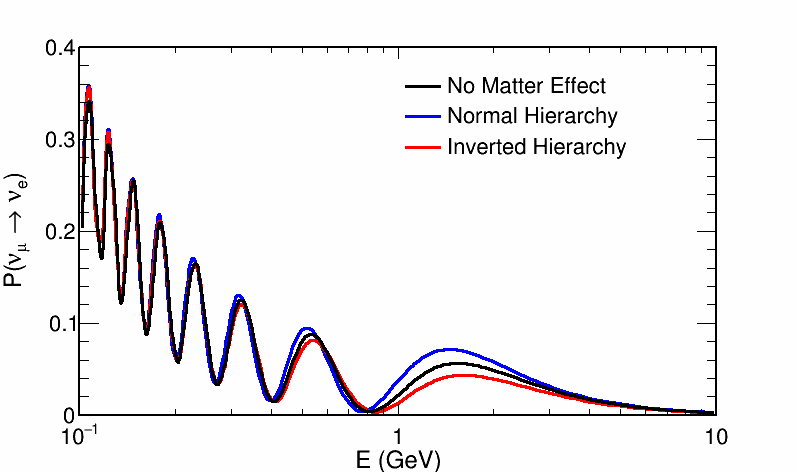
\includegraphics[width=.47\textwidth]{figures/MuE.png} &
    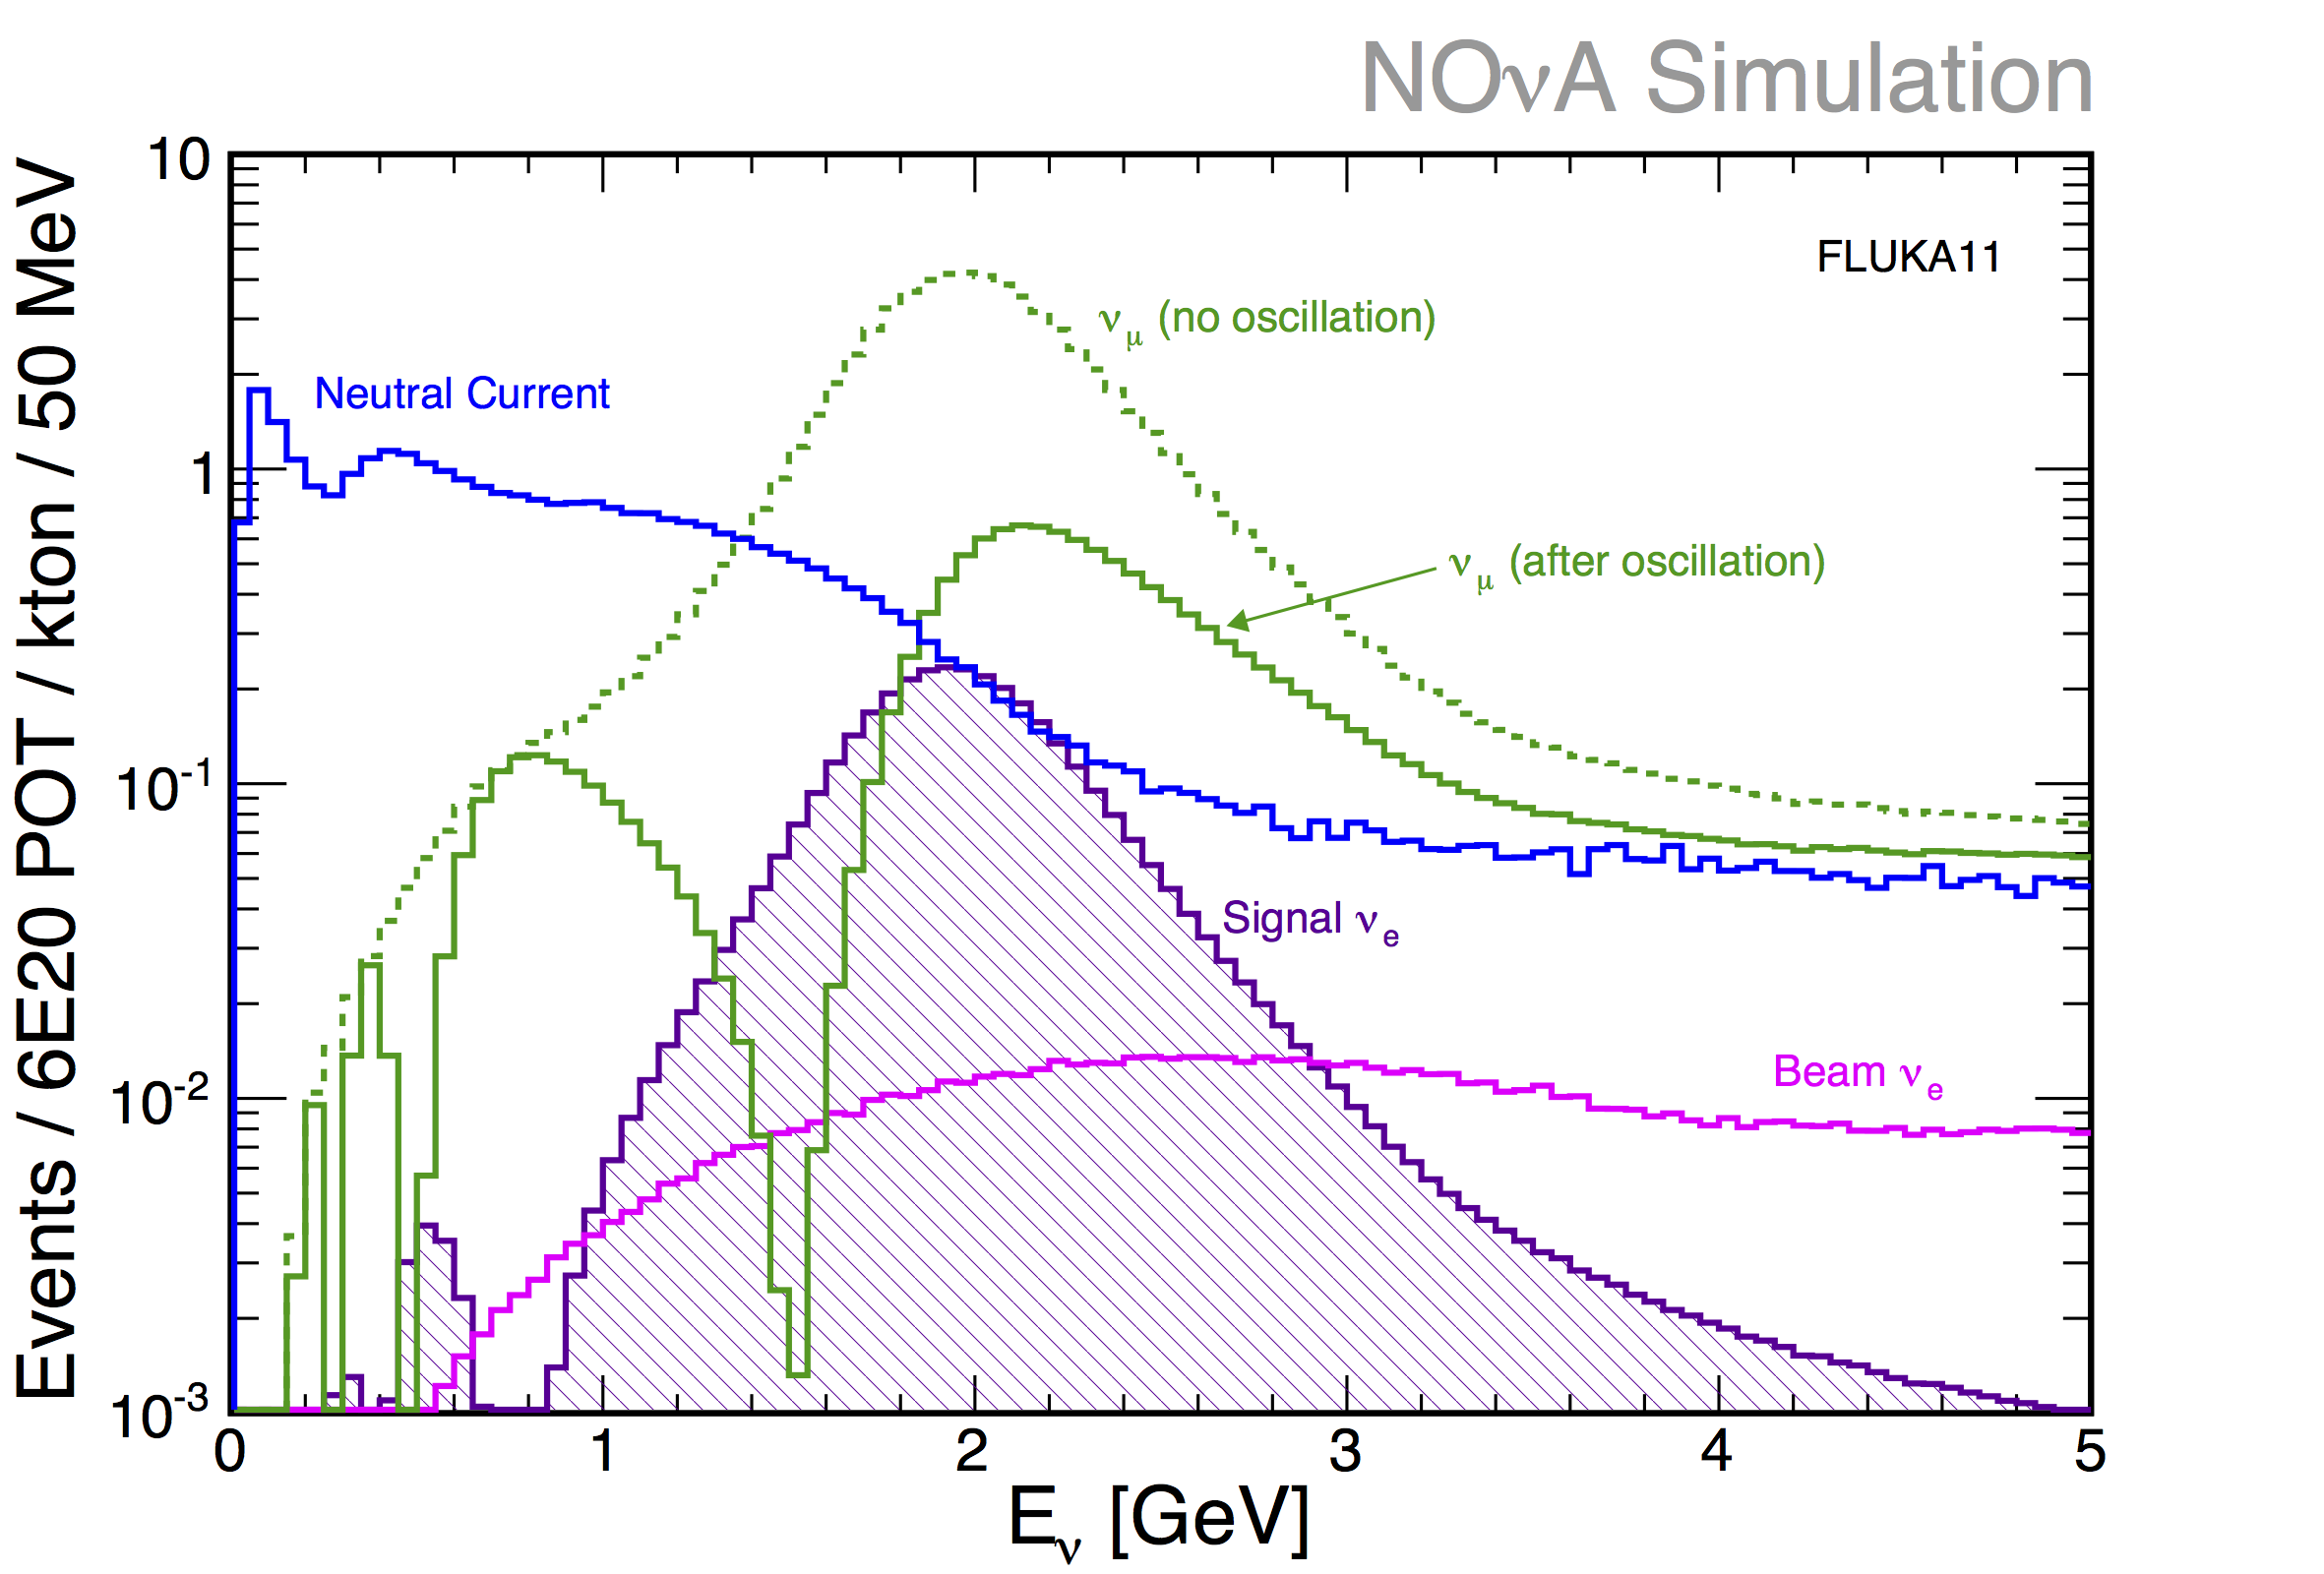
\includegraphics[width=.47\textwidth]{figures/BeamFluxXSec.png} \\
  \end{tabular}
  \caption[Probability of $\nue$ Appearance and Expected Event Rates for \nova]{Left: the probability of $\nue$ appearance. The probabilities are calculated assuming standard three flavor oscillations using the relevant values shown in table \ref{tab:LOverEValues}, except for $\delta_{CP}$ which is here set to $3\pi/2$. Right: The expected number of events as a function of true neutrino energy (with the exception of NCs), for individual components. The NC component is shown as a function of true visible energy $E_{vis} \equiv E_\nu \times y_{Bj}$, where $y_{Bj}$ is the fractional energy loss Bjorken scaling variable.}
  \label{fig:PMuEFluxXSec}
\end{figure}

As with the main \nova~analyses, the off-axis nature of the experiment has both pros and cons when searching for sterile oscillations via NC disappearance. Obviously a reduced neutrino flux is not great when searching for neutrino interactions. However, the CC backgrounds are highly suppressed due to oscillations, even with the $\nue$ appearance. This makes the selection of a relatively pure sample of NC events at the FD a much easier task.

\section{\texorpdfstring{The \nova~Detectors}{The NOvA Detectors}}

The \nova~Detectors are highly segmented, liquid scintillating calorimeters. They consist of PVC plastic cells filled with a liquid scintillating solution, and the active scintillating material makes about $65\%$ of the detectors by mass. The two detectors are functionally identical in order to reduce the effect of systematic errors, with the ND used to constrain the neutrino beam flux and energy and the FD used to measure the oscillated neutrino spectrum. This section first describes the general detector design, and later focuses on the specific details of the individual detectors. The information contained here is largely a summary of the \nova~TDR \cite{ref:TDRNOvA}, which contains a much more detailed account of the detectors. 

The basic structure of the \nova~detectors is a set of PVC plastic cells arranged together as planes and alternating in orientation. The cross section of the cells is approximately rectangular with dimensions of $4\unit{cm} \times 6\unit{cm}$. The cell length spans the entire height or width of the particular detector, depending on the orientation of the given plane. The PVC is extruded in groups of $16$ cells, as shown in figure \ref{fig:DetExtrusion}. Two extrusions are glued together to create a `module,' shown in figure \ref{fig:DetModule}. Many modules are glued together side by side to form a single plane. The planes are oriented such that the NuMI beam direction is approximately parallel to the plane normal vector.
\begin{figure}[htb]
  \centering
  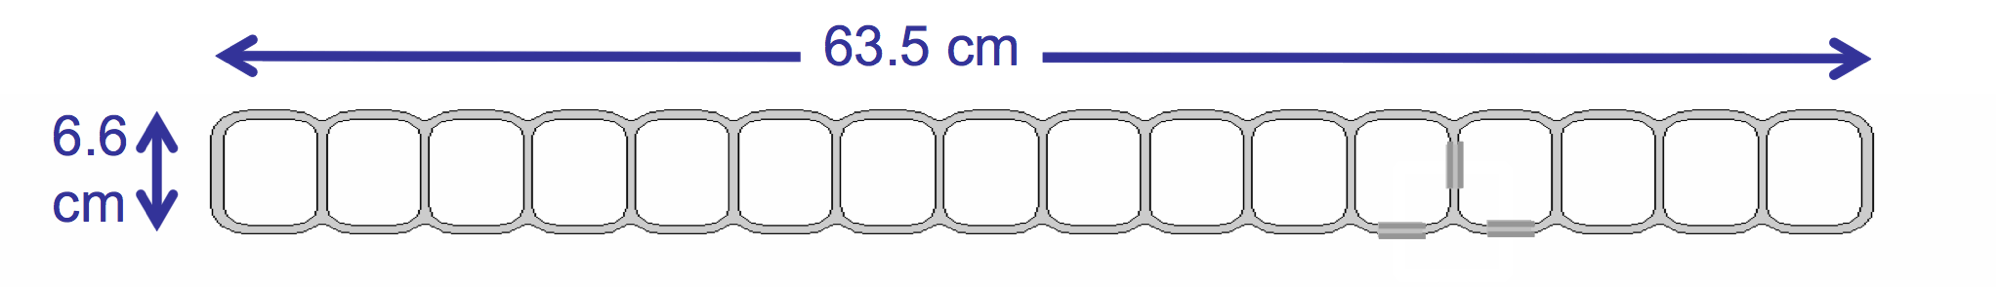
\includegraphics[width=0.75\textwidth]{figures/DetExtrusion.png}
  \caption[A PVC Extrusion]{A schematic of a PVC cell extrusion. The PVC is extruded along the axis into the page with a length equal to the detector height or width. Figure from \cite{ref:TDRNOvA}.}
  \label{fig:DetExtrusion}
\end{figure}

\begin{figure}[htb]
  \centering
  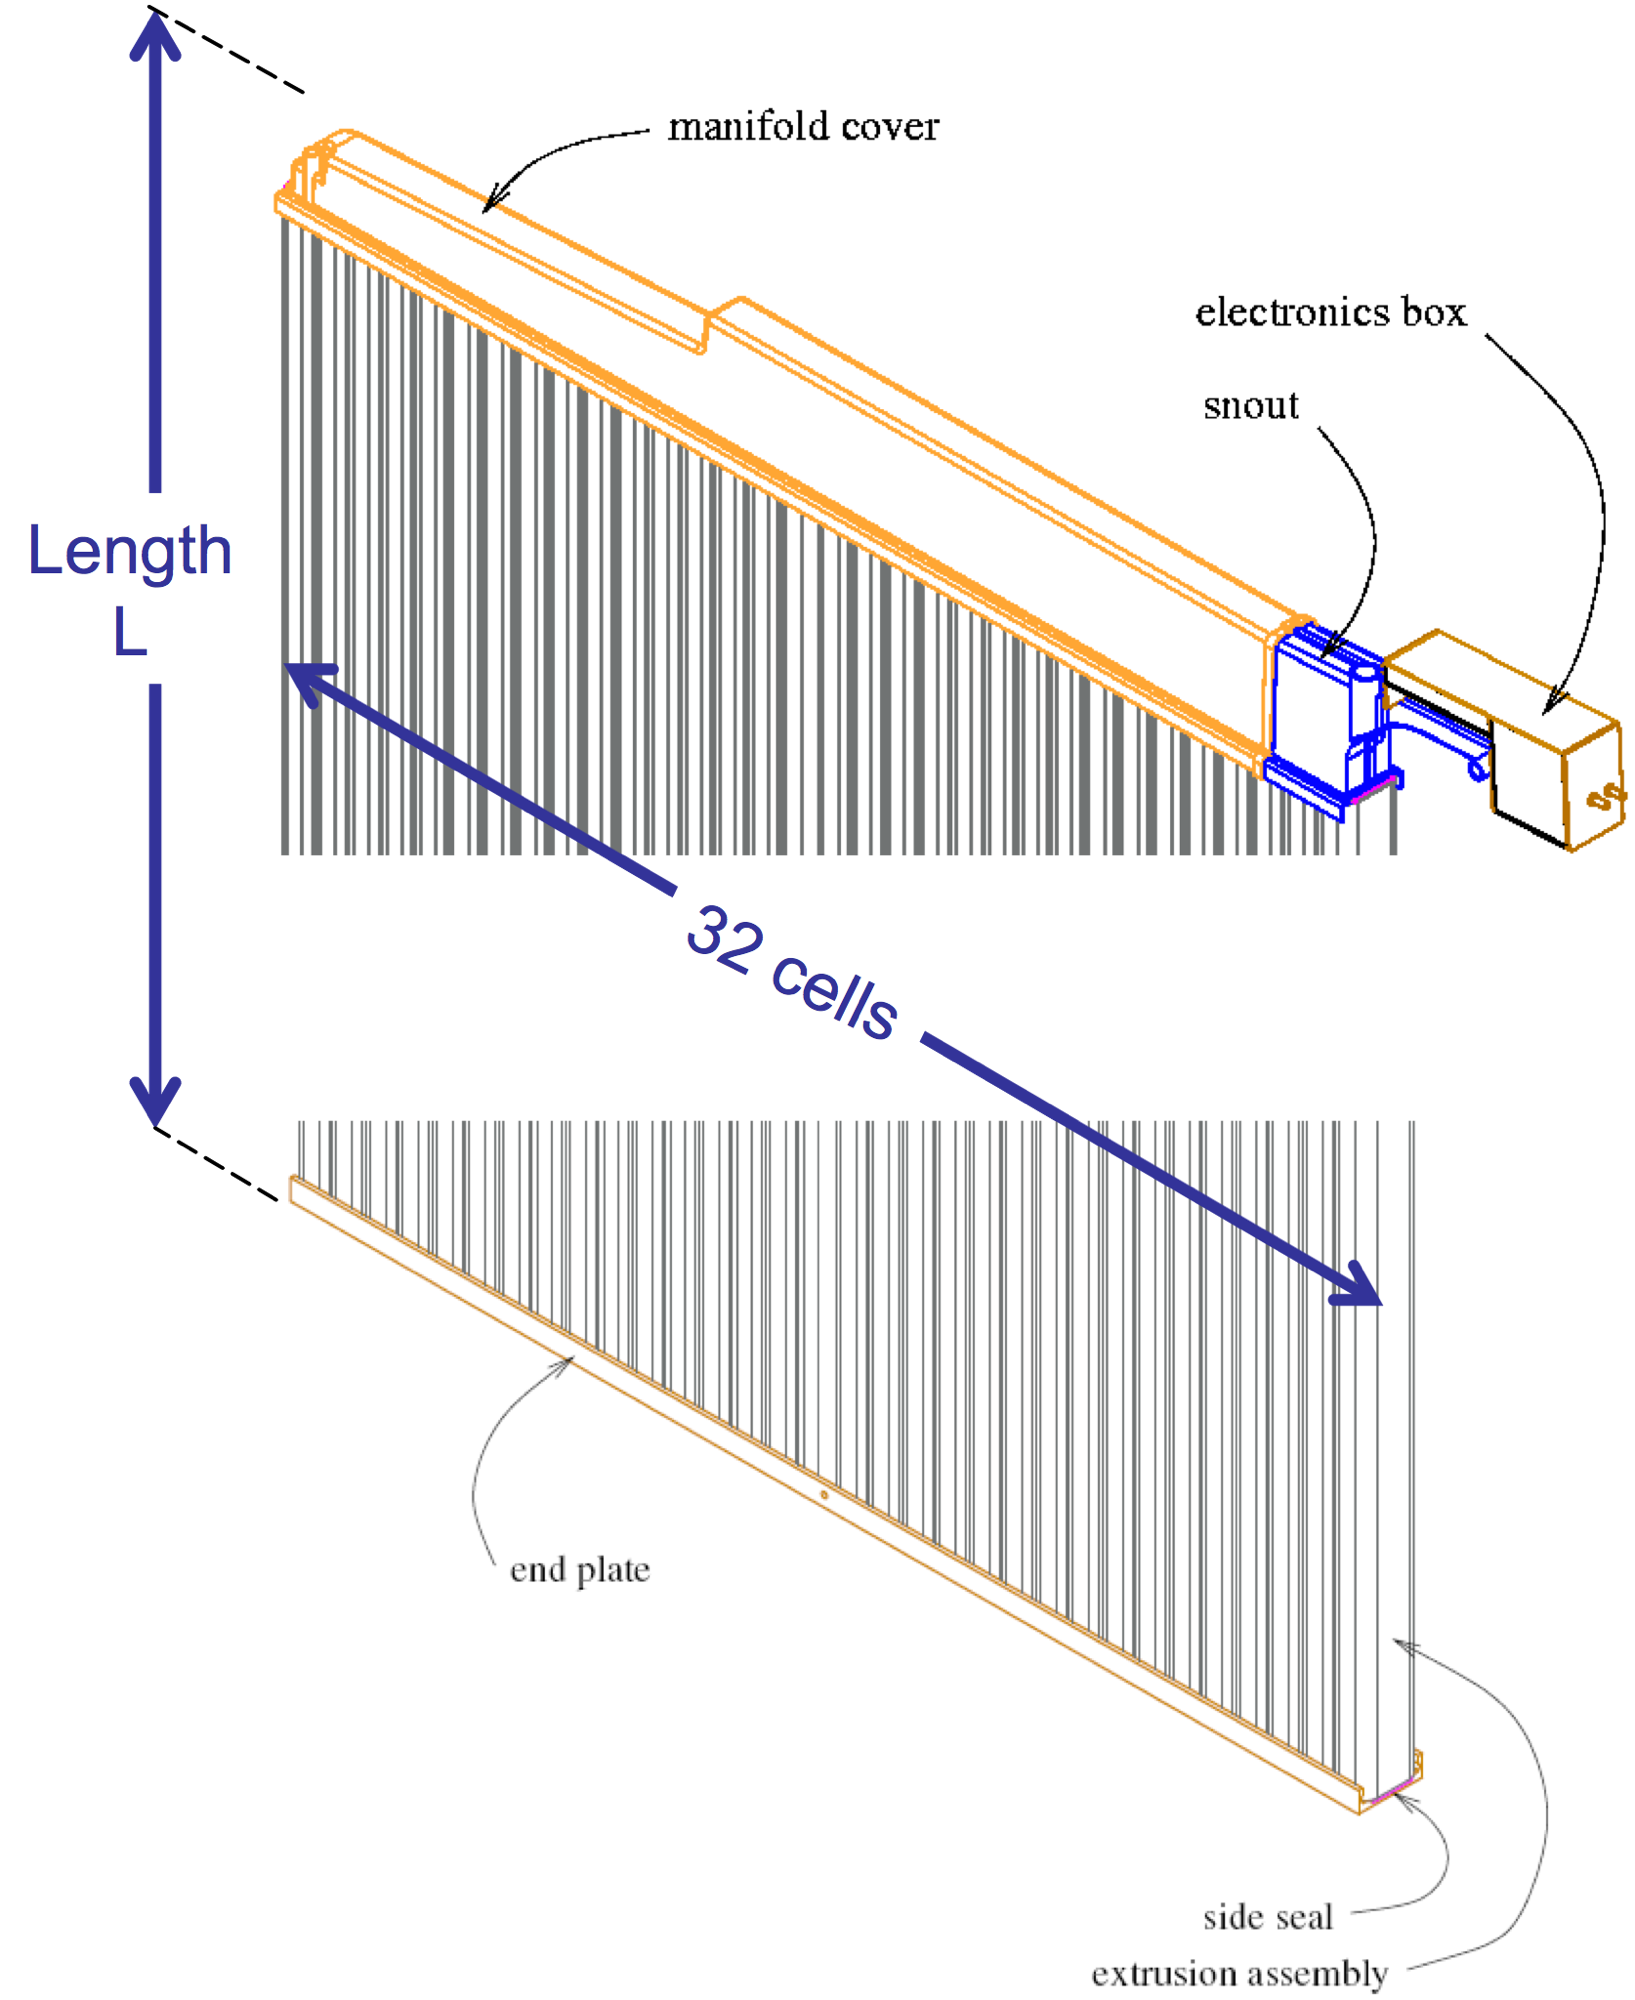
\includegraphics[width=0.75\textwidth]{figures/DetModule.png}
  \caption[A Detector Module]{A schematic of a module. A full plane is made up of modules connected side by side. Figure from \cite{ref:TDRNOvA}.}
  \label{fig:DetModule}
\end{figure}

The local detector coordinate systems consider the NuMI beam direction as the Z axis, height (or altitude) as the Y axis, and the X axis is the other remaining. As the NuMI beam points approximately to the north, the direction of positive X happens to point west. (The beam travels in the positive Z direction, and the positive Y direction points to higher elevation.) In this frame, a given plane can either locate activity in an XZ plane if the cells are in the vertical orientation, or a YZ plane if the cells are in the horizontal orientation. For this reason, the planes alternate between horizontal and vertical orientations to give a full three dimensional view of detector activity.

Each cell is filled with a liquid scintillator solution that consists of several different compounds, each with a specific function. Pseudocumene ({1,2,4-Trimethylbenzene}) is the scintillant used in the solution. The solution contains two wave shifters, PPO (2,5-Diphenyloxazole) and bis-MIS (1,4-bis(2-methylstyryl)\linebreak benzene). A small amount of Stadis-425 is used in the solution as an antistatic agent, and a small amount of tocopherol (Vitamin E) is added as an antioxidant. Mineral oil provides the solvent for each of the above compounds and makes up the majority of the solution. Table \ref{tab:scintillator} summarizes the solution contents and lists their mass fractions. The resultant mixture produces scintillation light in the low wavelength UV region, and shifts this to the violet-blue region.
\begin{table}[h]
  \begin{center}
    \begin{tabular}{c c c}
      \hline\hline
      Compound & Purpose & Mass Fraction \\
      \hline
      Mineral Oil & Solvent & $95.8\%$ \\
      Pseudocumene & Scintillant & $4.1\%$ \\
      PPO & Waveshifter & $0.091\%$ \\
      bis-MSB & Waveshifter & $0.0013\%$ \\
      Stadis-425 & Anti-static & $0.0003\%$ \\
      Vitamin E & Antioxidant & $0.0010\%$ \\
      \hline
    \end{tabular}
    \caption[Scintillator Solution Summary]{A summary of each component in the scintillation solution. Adapted from \cite{ref:TDRNOvA}.}
    \label{tab:scintillator}
  \end{center}
\end{table}

To collect the scintillation light, the inside of each cell is coated with titanium dioxide and a loop of a plastic wavelength shifting (WLS) fiber rests inside each cell. The TiO\textsubscript{2} is used as a reflective agent to maximize the scintillation light collection. A fluorescent dye in the WLS fiber absorbs this scintillation light and shifts it to the blue-green region. This light is then transmitted through the fiber to electronics for readout. A complete schematic of a cell is shown in figure \ref{fig:DetCell}.
\begin{figure}[htb]
  \centering
  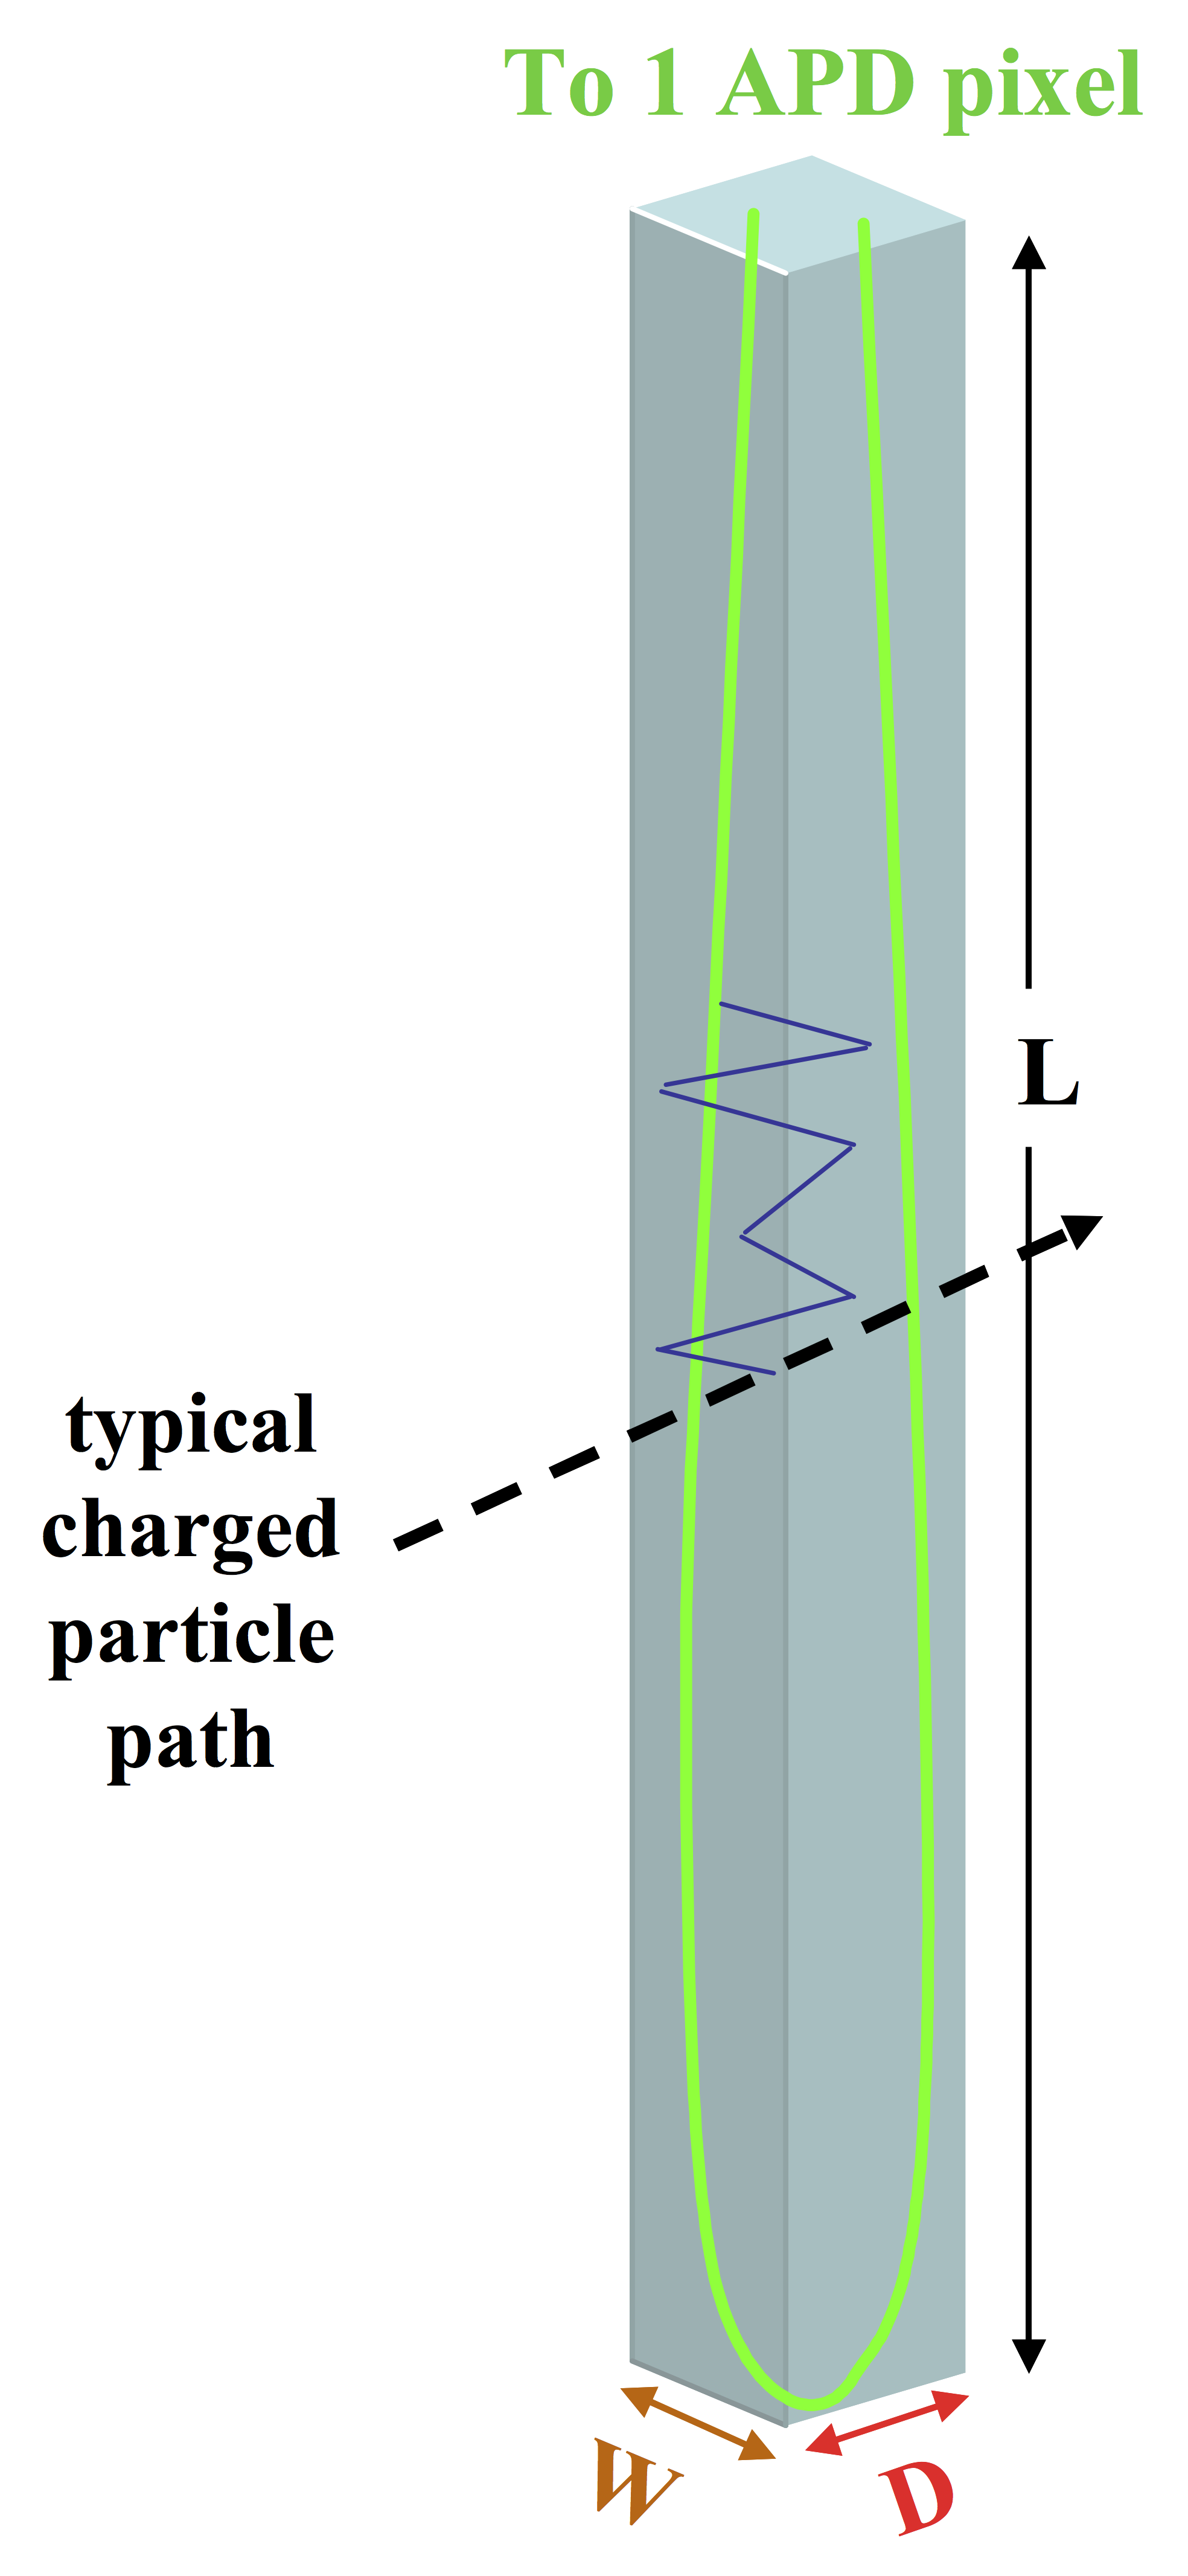
\includegraphics[width=0.2\textwidth]{figures/DetCell.png}
  \caption[A Detector Cell]{A schematic of the inside of a cell. The width and depth are approximately $W \approx 4\unit{cm}$ and $D \approx 6\unit{cm}$, respectively. The green curve is the WLS fiber, and the zigzagging blue line is a path light might take from emission by the scintillator through absorption by the WLS fiber. Figure from \cite{ref:TDRNOvA}.}
  \label{fig:DetCell}
\end{figure}

The first component in data readout is collection and amplification by a Hamamatsu avalanche photodiode (APD). A single APD collects the light from all 32 cells in a module, collecting light from both ends of the WLS fiber. Figure \ref{fig:DetAPD} shows an APD and the ends of the WLS fibers set in a mount to be placed next to the APD. APDs were chosen over PMTs due to their high quantum efficiency, especially for green light. This is shown in figure \ref{fig:APDvsPMT} against the light output of the WLS fibers.
\begin{figure}[htb]
  \centering
  \begin{tabular}{c c}
    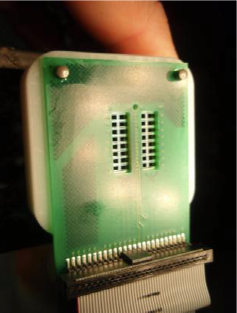
\includegraphics[width=.47\textwidth]{figures/DetAPD.png} &
    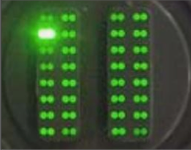
\includegraphics[width=.47\textwidth]{figures/DetFiberEnd.png} \\
  \end{tabular}
  \caption[An APD]{Left: An APD. Right: The ends of 32 WLS fibers that will be pressed against the APD face shown on the left.}
  \label{fig:DetAPD}
\end{figure}

\begin{figure}[htb]
  \centering
  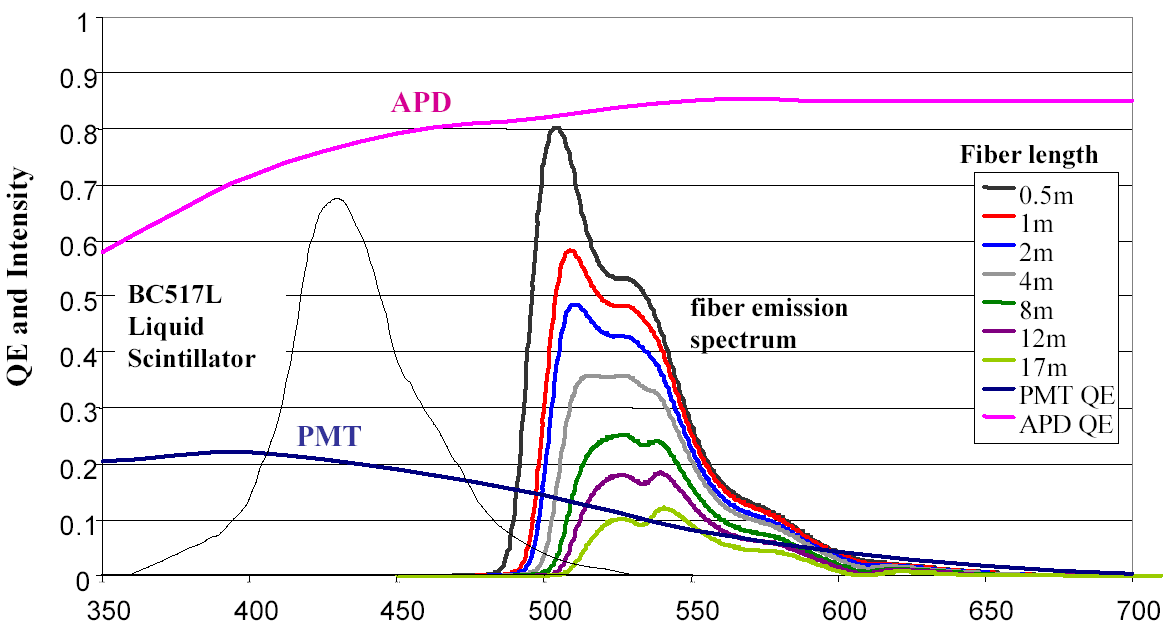
\includegraphics[width=0.95\textwidth]{figures/APDvsPMT.png}
  \caption[Quantum Efficiency of APDs and Light Intensity Output of WLS fibers]{Quantum efficiency of APDs as a function of light wavelength. For comparison, the QE of PMTs is shown in navy. The light output of the liquid scintillator is shown in the thin, black curve. The light output for the WLS fibers is also shown for a variety of different lengths through the fiber. The intensities are in arbitrary units. While the blue light is almost fully attenuated through the fiber, the green light is only modestly attenuated. Figure from \cite{ref:TDRNOvA}.}
  \label{fig:APDvsPMT}
\end{figure}

Each APD is connected directly to a thermoelectric cooler and housed in an electronics box as shown in figure \ref{fig:DetModule}. The cooler keeps the operating temperature for the APD at $-15^\circ$ to reduce noise. The APDs are held at a voltage of about $425\unit{V}$ to run at a gain of $100$, though exact voltages are set individually. In October 2015, the gain for the FD APDs was increased to 150 to be more sensitive to light from the far ends of the fibers. The thermoelectric cooler is part of a larger front-end board (FEB) that is also housed inside the same electronics box as the APD. The FEB thus provides the cooling and voltage for the APD, but it also digitizes the signals from the APD.

The electronics for the \nova~detectors were installed in 64 plane sections called diblocks. The signals from (up to) 64 FEBs are read out by a single data concentrator module (DCM). Due to the alternating orientations of the planes, and thus the modules, electronics boxes are found on either the top or one side of the detector. Consequently, a given DCM does not read out one FEB per plane, but rather (up to) two FEBs per plane. The two FEBs are always from adjacent modules, and the modules always share the same X or Y coordinate range based on the module orientation. This diblock structure is important because it allowed for data collection at the FD before the detector was fully commissioned.

Data stored by the DCMs are stored in $50\microsec$ blocks called microslices, which are transferred to a data buffer farm in larger $5\unit{ms}$ blocks called millislices. Data is stored in the farm for up to $20$ minutes before being erased. During this time, different trigger decisions can be applied to keep the data for different purposes such as recording beam activity, searching for good calibration candidates, or searching for exotic physics like monopoles. Data that pass a trigger decision are written to disk and permanently stored, and this mechanism allows the FEBs to collect data continuously.

Detector activity that could be due to a beam event is captured within a $500\microsec$ window. These events are specifically triggered by a signal from Fermilab, corrected for time of flight at the FD. The event window is centered around the ${\sim}10\microsec$ beam spill, which allows for considerable drift in the timing systems without loss of data \cite{ref:ThesisEvan}. Other $500\microsec$ event windows without beam candidates are stored as cosmic trigger data that are useful for predicting the cosmic background event rate.

Data are collected by organizing these events into larger run and subrun file structures. Subruns are populated with events until either a maximum file size is reached, or after an hour of data taking has elapsed, whichever comes first. Runs are comprised of $64$ subruns for the FD, and $24$ subruns for the ND, and are numbered in succession such that larger numbered runs correspond to later times.

\subsection{Far Detector}

The \nova~FD is situated $810\unit{km}$ from the beam target in Ash River, MN. Both the horizontal and vertical planes consist of $12$ modules, or $384$ cells, for a total cross sectional area of about $15.2\unit{m} \times 15.2\unit{m}$. The fully commissioned detector has $14$ diblocks (data taking began with as few as $4$), or $896$ planes, with a total length of about $59.6\unit{m}$. This means that the detector reads out $344$,$064$ individual cells, or channels. The FD weighs $14\unit{kT}$, which is about $65\%$ scintillator and $35\%$ PVC plastic.

The detector itself is inside a building that is at the surface, mostly dug underground and partially above ground. The site is at an elevation of about $1220\unit{ft}$ and thus subject to a large background of cosmic rays. A large amount of overburden is used to mitigate this effect. $2.5\unit{ft}$ of precast concrete covers the entire detector and is capped with $1.5\unit{ft}$ of concrete cast in place. Finally, $6$" of barite, or barium sulfate, is placed above the concrete and composed of loosely packed rocks. Barite was chosen because it is a high Z material with a high stopping power for cosmic ray photons. Together, the concrete and barite provide around $14$ radiation lengths for the cosmic rays. Figure \ref{fig:FD} shows the FD and the building inside which it is located.
\begin{figure}[htb]
  \centering
  \begin{tabular}{c c}
    \includegraphics[width=.29\textwidth]{figures/NOvAFD.jpg} &
    \includegraphics[width=.65\textwidth]{figures/NOvAFDSite.jpg} \\
  \end{tabular}
  \caption[The \nova~Far Detector]{Left: The \nova~FD. The beam comes from the back of the photograph and out of the page. The red and yellow structure is a piovter that was used to rotate and put the detector blocks into position and is not part of the detector. A person can be seen halfway up on the right of the detector for scale. Right: The FD building. The detector is beneath the rocky section on the right of the photograph, which only partially shows the barite overburden.}
  \label{fig:FD}
\end{figure}

Even with the overburden, it is still expected to see cosmic rays in the FD with a rate over $200\unit{kHz}$. This is the main reason why \nova~must use a trigger from the Fermilab accelerator to signal a beam event, but also why taking cosmic trigger data is so important. These data are used to develop and train cuts designed to remove cosmic background. Later, a predicted background is made from an independent sample, namely the data regions in the NuMI trigger events that fall safely outside the smaller beam window.

\subsection{Near Detector}

The \nova~ND is situated $1015\unit{m}$ from the beam target, on site at Fermilab. It is composed of two different sections, a fully active region much like the FD and a muon catcher. In the fully active region, each plane consists of $3$ modules, or $96$ cells, for a total cross sectional area of about $3.8\unit{m} \times 3.8\unit{m}$. The region is made up of $192$ planes with a length of about $12.7\unit{m}$ and corresponds to $3$ diblocks for the electronics. The NuMI beam first passes through this fully active region, but since it is so much shorter than the FD, the muon catcher is necessary to be able to accurately measure particle energies. For this section, planes of steel, which have an excellent stopping power for muons, are interspersed between the alternating planes. The energy loss of muons passing through steel is well known allowing for accurate event reconstruction. This region is specifically made of a horizontal plane, a $10\unit{cm}$ steel plane, and a vertical plane, repeated $11$ times for an additional $22$ active planes. However, for economic reasons the steel and planes in this region were recycled from a prototype near detector that was built using the original design of $3$ modules $\times 2$ modules. Thus, the planes in the muon catcher are as wide as the fully active region, but only $2/3$ as tall, at about $2.6\unit{m}$. In total, the ND is $15.8\unit{m}$ in length, has $20$,$192$ cells, and $214$ active planes. It weighs $290\unit{T}$, of which $130\unit{T}$ is scintillator, $81\unit{T}$ is PVC plastic, and $78\unit{T}$ is steel \cite{ref:NDMass}. Figure \ref{fig:ND} shows the ND from both beam directions, and table \ref{tab:Dets} summarizes the properties of both detectors.
\begin{figure}[htb]
  \centering
  \begin{tabular}{c c}
    \includegraphics[width=.47\textwidth]{figures/NOvAND.jpg} &
    \includegraphics[width=.47\textwidth]{figures/NOvANDMC.jpg} \\
  \end{tabular}
  \caption[The \nova~Near Detector]{The \nova~ND. Left: View from the side where the beam enters the detector. The red structure is a bookend and not part of the active detector. A person is seen on the right for scale. Right: View from the side where the beam exits the detector. The red and grey structure above the muon catcher is for worker access to this detector region and not part of the active detector.}
  \label{fig:ND}
\end{figure}

Unlike the FD, the ND is not a surface detector. It is located $105\unit{m}$ below the surface in the same underground cavern as the MINOS ND, as depicted in figure \ref{fig:DetNDPlan}. This means that the ND is not subject to a cosmic ray rate like FD. However, given the close proximity to the beam source, the ND can obverse multiple neutrino events in every beam spill. This leads to the potential for pileup, so the electronics for the ND were designed to sample the data $4$ times faster than the FD to deal with this.
\begin{figure}[htb]
  \centering
  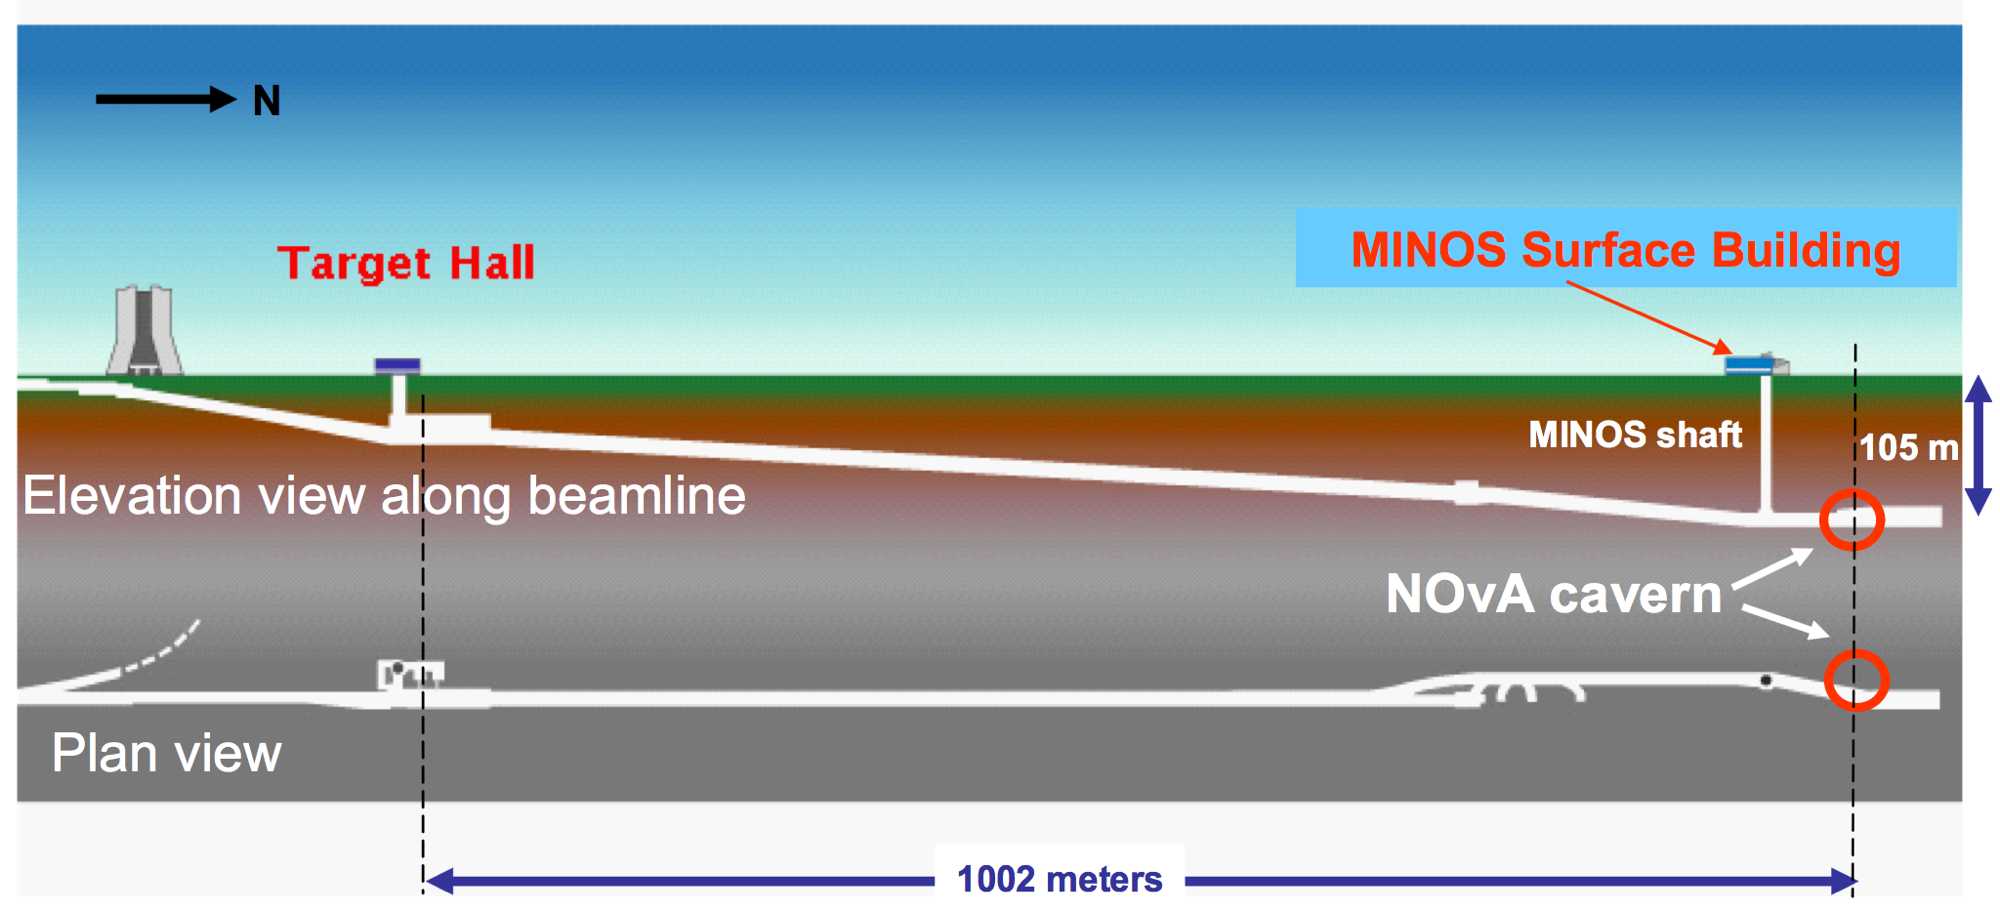
\includegraphics[width=0.75\textwidth]{figures/DetNDPlan.png}
  \caption[Schematic of the NuMI Beam line]{A schematic of the NuMI beam line, showing the location of the ND hall. Figure from \cite{ref:TDRNOvA}.}
  \label{fig:DetNDPlan}
\end{figure}

\begin{table}[htb]
  \begin{center}
    \begin{tabular}{c c c}
      \hline\hline
      Detector Property & FD & ND \\
      \hline
      Detector Weight (kT) & $14$ & $0.3$ \\
      Number of Diblocks & $8$ & $3$~(${+}$Muon Catcher) \\
      Number of Planes & $896$ & $214$ \\
      Number of Cells & $344064$ & $20192$ \\
      Detector Length (m) & $59.6$ & $15.8$ \\
      Detector Width (m) & $15.8$ & $4.2$ \\
      Detector Height (m) & $15.8$ & $4.2$~$(2.8)$ \\
      Cell Depth (cm) & $5.6$ & $5.6$ \\
      Cell Width (cm) & $3.6$ & $3.6$ \\
      Cell Length (m) & $15.2$ & $3.8$~($3.8$H,~$2.6$V$)$ \\
      \hline
    \end{tabular}
    \caption[Detector Properties]{A summary of the physical properties of both detectors. For the ND, a single value means the property is consistent across the entire detector. Otherwise, values in parenthesis are for the muon catcher only. Note that the detector width and height exceed the cell lengths due to inclusion of the end caps on either side of the planes.}
    \label{tab:Dets}
  \end{center}
\end{table}